% AASTeX v6.2
%\documentclass[preprint]{aastex62}

% ApJ Format
\documentclass[iop,revtex4,twocolumn,apj,numberedappendix,appendixfloats]{emulateapj}
\usepackage{apjfonts}
% Hyperlinks & Bookmarks
\usepackage[pagebackref=false,colorlinks=true,citecolor=blue,linkcolor=blue,breaklinks=true,bookmarks=true]{hyperref}
\usepackage{amsmath}
\usepackage{comment}

% Units
\newcommand{\kms}{km~s$^{-1}$}
\newcommand{\msun}{$M_{\odot}$}
\newcommand{\msunyr}{$M_{\odot}~{\rm yr}^{-1}$}
\newcommand{\lsun}{$L_{\odot}$}
\newcommand{\ergs}{erg~s$^{-1}$}
\newcommand{\cmsq}{cm$^{-2}$}
\newcommand{\um}{$\mu$m}
\newcommand{\uJy}{$\mu$Jy}
\newcommand{\sqdeg}{deg$^2$}
\newcommand{\lx}{$L_{\rm X}$}
\newcommand{\lmir}{$L_{\rm 12\mu m}$}
\newcommand{\loiii}{$L_{\rm [OIII]}$}
% special 
\newcommand{\nod}{\nodata}
\newcommand{\chandra}{{\it Chandra}}
\newcommand{\xmm}{{\it XMM-Newton}}
% citations
\defcitealias{Fu15a}{Paper I} 
\defcitealias{Fu15b}{Paper II}

\usepackage{epstopdf}

\begin{document}

\title{Chandra Observations of Radio-Selected Dual Active Galactic Nuclei in Stripe 82}

\author{
Arran C. Gross\altaffilmark{1}, 
Hai Fu\altaffilmark{1}, 
A. D. Myers\altaffilmark{2},
J. M. Wrobel\altaffilmark{3}, and
S. G. Djorgovski\altaffilmark{4}
}
\altaffiltext{1}{Department of Physics \& Astronomy, The University of Iowa, 203 Van Allen Hall, Iowa City, IA 52242}
\altaffiltext{2}{Department of Physics \& Astronomy, University of Wyoming, Laramie, WY 82071}
\altaffiltext{3}{National Radio Astronomy Observatory, P.O. Box O, 1003 Lopezville Road, Socorro, NM 87801}
\altaffiltext{4}{California Institute of Technology, 1200 E. California Blvd., Pasadena, CA 91125}

\begin{abstract}
Merger simulations predict that tidally induced gas inflows can trigger kiloparsec-scale dual active galactic nuclei (dAGNs) when both supermassive black holes (SMBHs) in a merger accrete simultaneously. Previously with the Very Large Array, we have confirmed four dAGNs with redshifts between $0.04 < z < 0.22$ and projected separations between 4.3 and 9.2 kpc in the SDSS Stripe 82 field. Here we present \chandra\, observations of these dAGNs and compare their multi-wavelength properties with those of single and dual AGNs from the literature. We detect six of the AGNs and obtained 3$\sigma$ upper limits for the remaining two. The rest-frame $2-10$\,keV luminosities range between $39.8 < \log L_{\rm X}/{\rm erg\,s^{-1}} < 42.0$. Combined with their 5\,GHz and H$\alpha$ luminosities, we find that our dAGNs have properties similar to the radio-loud low-luminosity AGNs and Seyferts in nearby galaxies. Furthermore, we estimate the SMBH masses for our sample using the $M_{\rm BH}-\sigma_\star$ relation, and find that our dAGNs agree well with the Black Hole Fundamental Plane of $L_{\rm 5GHz}$, $L_X$ and $M_{\rm BH}$ and have Eddington ratios between $-5.5 < \log L_{\rm bol}/L_{\rm Edd} < -3.0$. Finally, we estimate nuclear obscuration of our dAGNs using the X-ray hardness ratio, the X-ray-to-[O\,{\sc iii}] luminosity ratio, and the X-ray-to-12$\mu$m luminosity ratio. For three of the six X-ray detections, we estimate the intrinsic column density to be between $21.2 < \log N_{\rm H}/{\rm cm^{-2}} < 22.7$ based on the X-ray hardness ratio and an assumed intrinsic photon index of $\Gamma = 1.9$; for the remaining three detections, the hardness ratios are consistent with no obscuration. A statistical test between the distributions of hardness ratios of our sample and a comparison sample of similar luminosity isolated AGNs reveals no significant differences. Considering the  contribution from star formation to the [O\,{\sc iii}] and mid-IR luminosities, we find no convincing evidence that the dAGNs are more obscured than comparable AGNs in the general population, in contrast to the predictions from merger simulations. To reconcile the high AGN duty cycle in mergers and the lack of nuclear obscuration, we suggest that the dAGNs may have been triggered by minor tidal perturbations instead of massive gas inflows. 
\end{abstract}

\keywords{galaxies: active --- galaxies: nuclei --- galaxies: interactions}

\section{Introduction} \label{sec:intro}

In a universe dominated by cold dark matter and dark energy, galaxies are built up from a series of major and minor mergers. Cosmological hydrodynamical simulations have shown that galaxies like our Milky Way have acquired a large ex-situ component from a number of other galaxies during the cosmic history \citep[e.g., ][]{Rodriguez-Gomez16,Pillepich18}. Zooming in on the encounter, idealized merger simulations have predicted that gravitational torques from tidally-induced stellar bars can drive large amounts of interstellar gas to the central kiloparsec on short timescales. The sudden gas inflow could dilute gas metallicity in the interstellar medium, fuel nuclear starbursts, and even trigger supermassive black hole (SMBH) accretion in the central parsec \citep[e.g.,][]{Barnes91,Torrey12,Capelo17a}. As a result, simultaneous SMBH accretion could occur at the smallest, sub-galactic separations ($\lesssim$10\,kpc) when the tidal force is strongest \citep[e.g.,][]{Van-Wassenhove12,Blecha13,Rosas-Guevara18}. Mergers in this stage would appear as kpc-scale dual active galactic nuclei (dAGN) before nuclear coalescence. The dynamical friction timescale for $r < 10$\,kpc is comparable to the \citet{Salpeter64} $e$-folding timescale for Eddington-limited black hole growth ($\tau_{\rm Sal} = 45 {\rm Myr} (\eta_{\rm rad}/0.1)$, where $\eta_{\rm rad}$ is the radiative efficiency) and it is in the middle of the wide range of estimated AGN lifetimes from different methods ($\tau_{\rm AGN} \sim 1-100$\,Myr; \citealt{Martini04,Hopkins05a}). Therefore, kpc-scale binary AGNs could offer useful constraints on the average duration of an AGN episode.

The first example of a kpc-scale dAGN is probably the radio galaxy 3C\,75 \citep{Owen85}, which shows a pair of radio jets originating from a pair of stellar nuclei separated by 7.7\,kpc. Detailed case studies have identified a number of kpc-scale dAGNs with optical and X-ray data, including LBQS\,0103$-$2753 \citep{Junkkarinen01}, NGC\,6240 \citep{Komossa03}, 3C\,294 \citep{Stockton04}, Arp\,299 \citep{Ballo04}, Mrk\,463 \citep{Bianchi08}, NGC\,3393 \citep{Fabbiano11}, and Mrk\,266 \citep{Mazzarella12}.
%
To assemble a statistical sample of dAGNs with well-understood selection biases, various techniques have been developed to identify dAGN candidates and to confirm these candidates systematically. 
%
Effective candidate identification involves lower-resolution observations of larger samples: (1) double-peaked [O\,{\sc iii}] AGNs in the DEEP2 Galaxy Redshift Survey \citep{Gerke07,Comerford09a} and in the Sloan Digital Sky Survey \citep[SDSS;][]{Wang09,Liu10a,Smith10}, (2) hard-X-ray-detected nearby AGNs in the Swift Burst Alert Telescope (BAT) survey \citep{Koss10}, (3) radio AGN pairs in the VLA Stripe 82 survey \citep{Fu15a}, (4) mid-IR-color-selected AGNs in WISE \citep{Satyapal14,Satyapal17}, (5) BPT-selected AGNs in spectroscopic galaxy pairs in SDSS \citep{Ellison11,Liu12,Fu18}, and (6) the \chandra \ survey of merging galaxies \citep{Brassington07,Teng12}.
%
Robust candidate confirmation involves high-resolution observations at wavelengths that trace AGN activity, e.g., in optical and near-IR with Keck adaptive optics imaging \citep{Fu11a,Rosario11}, \textit{HST} imaging \citep{Liu13,Comerford15,Liu17c}, and integral-field spectroscopy \citep{McGurk11,Fu12a}, in X-ray with \chandra \,\citep{Comerford11,Koss11,Koss12,Teng12,Liu13a,Comerford15,Ellison17} and NuStar \citep{Ptak15,Koss16}, and in radio with the Very Large Array \citep{Fu11b,Fu15b,Muller-Sanchez15} and the Very Long Baseline Array \citep{Tingay11,Deane14,Wrobel14,Bondi16,Liu17b}.
%
Identifying and confirming dAGNs is a slow process; currently there are only a total of $\sim$30 dAGNs with projected separations less than 10\,kpc in the literature \citep[see][for a compilation]{Satyapal17}. Despite the small sample, it seems clear that the AGN duty cycle is significantly higher in mergers than in isolated systems. 

X-ray observations can provide an effective measure of the accretion power of the SMBHs. Nuclear X-ray emission in the keV-band could be produced by several mechanisms related to accretion: (1) inverse-Compton scattered thermal emission from a hot ($\sim10^9$\,K) corona \citep{Liang77,Haardt93} embedded in a cooler ($\sim10^5$\,K) standard geometrically-thin optically-thick disk \citep{Shakura73}, (2) a hot ($\sim10^{12}$\,K at the Schwarzschild radius) advection-dominated accretion flow \citep[ADAF; see][for a review]{Yuan14}, and (3) synchrotron and self-Comptonized emission from radiative shocks at the base of relativistic jets \citep{Yuan02}. Although it is difficult to disentangle the contribution of the various mechanisms in individual AGNs, generally speaking, the ``disk-corona'' model produces the ``big blue bump'' in the UV and soft X-ray and likely dominates at high accretion rates ($L_{\rm bol}/L_{\rm Edd} > 0.01$), while the ADAF and the ``disk-jet'' models at low accretion rates ($L_{\rm bol}/L_{\rm Edd} < 0.01$). 
%
At low X-ray luminosity ($\lesssim 10^{42}$\,\ergs), another complication arises: nonnuclear host-galaxy X-ray emission on kpc scales can be confused with nuclear emission in distant galaxies. Such emission may appear spatially {\it unresolved} at the \chandra\ resolution at $z \gtrsim 0.05$, where $1\arcsec\ \gtrsim 1$\,kpc. Common nonnuclear X-ray emission from normal galaxies originate from (1) the hot ISM in hydrostatic equilibrium (often seen in early-type galaxies; e.g., \citealt{Forman85}) and (2) X-ray binaries, SNe remnants, and hot winds produced by recent star formation (often seen in late-type galaxies and starburst galaxies; e.g., \citealt{Fabbiano89}). Such spatially extended X-ray emission have typical luminosities between $10^{38}$ and $10^{42}$\,\ergs, approaching the level of nuclear X-ray luminosity in Seyferts ($10^{42} < L_{\rm 0.5-10 keV} < 10^{44}$\,\ergs; \citealt{Brusa07}). 

Nuclear X-ray emission can be effectively obscured by Helium and heavier elements due to photoelectric absorption \citep{Morrison83}. The obscuration can be caused by a dusty molecular torus at $\sim$10-pc scales and the intervening ISM in the host galaxy. The former is suggested by the AGN unification scheme \citep{Urry95} and confirmed in observations of narrow-line FR\,II radio galaxies \citep[e.g.,][]{Sambruna99} and nearby Seyferts \citep[e.g.,][]{Garcia-Burillo16,Gallimore16,Alonso-Herrero18,Fabbiano18}. But the torus may be absent at low accretion rates, such as the FR\,I radio galaxies in the 3CR sample \citep[e.g.,][]{Donato04,Balmaverde06,Evans06a} and the nearby LLAGNs \citep[e.g.,][]{Ho08}. In these cases, X-ray emission can only be obscured by the intervening ISM \citep[e.g.,][]{Gilli14}. Because the gas column density is elevated during a galaxy merger by tidally induced gas inflows, one would expect an excess of obscured AGNs in late-stage mergers \citep[e.g.,][]{Hopkins05a}.

In this series, we identify dAGNs candidates with the wide-area 2\arcsec-resolution VLA 1.4\,GHz survey of the Stripe 82 field \citep[][hereafter \citetalias{Fu15a}]{Fu15a} and confirm these candidates with optical spectroscopy and 0.3\arcsec-resolution VLA 6\,GHz observations \citep[][hereafter \citetalias{Fu15b}]{Fu15b}. Powered by \chandra X-ray observations of the VLA-confirmed dAGNs, here we mainly address two questions: {\it Do dAGNs follow the same multi-wavelength scaling relations as the general AGN population?} As well,{\it \, are dAGNs obscured to a similar degree as the general AGN population?} 
%
This paper is organized as follows. In \S~\ref{sec:obs} we describe the \chandra\ observations and data reduction procedures. In \S\,\ref{sec:analysis} we present the X-ray photometry and spectral fitting procedures. We synthesize our previous observations and the deduced X-ray properties of the dAGNs in \S~\ref{sec:results}, where we test whether the dAGNs deviate from the scaling relations established by general AGNs of similar luminosities and also address whether dAGNs are potentially more obscured at X-ray wavelengths.  
We conclude with a summary of our results and discuss their implications in \S~\ref{sec:summary}.
% possibility that dAGNs are triggered by merger-induced stochastic feeding instead of large-scale gas inflows 
%
Throughout, we adopt a $\Lambda$CDM cosmology with $\Omega_{\rm m} = 0.3, \ \Omega_{\Lambda} = 0.7$, and $h$ = 0.7. As usual, the spectral index $\alpha$ and the photon index $\Gamma$ are defined such that $F_\nu \propto \nu^{-\alpha}$ and $n(E) \propto E^{-\Gamma}$.

%%%%%%%%%%%%%%%%%%%%%%%

\section{Chandra Observations} \label{sec:obs}

\begin{figure*}[!t]
\centering
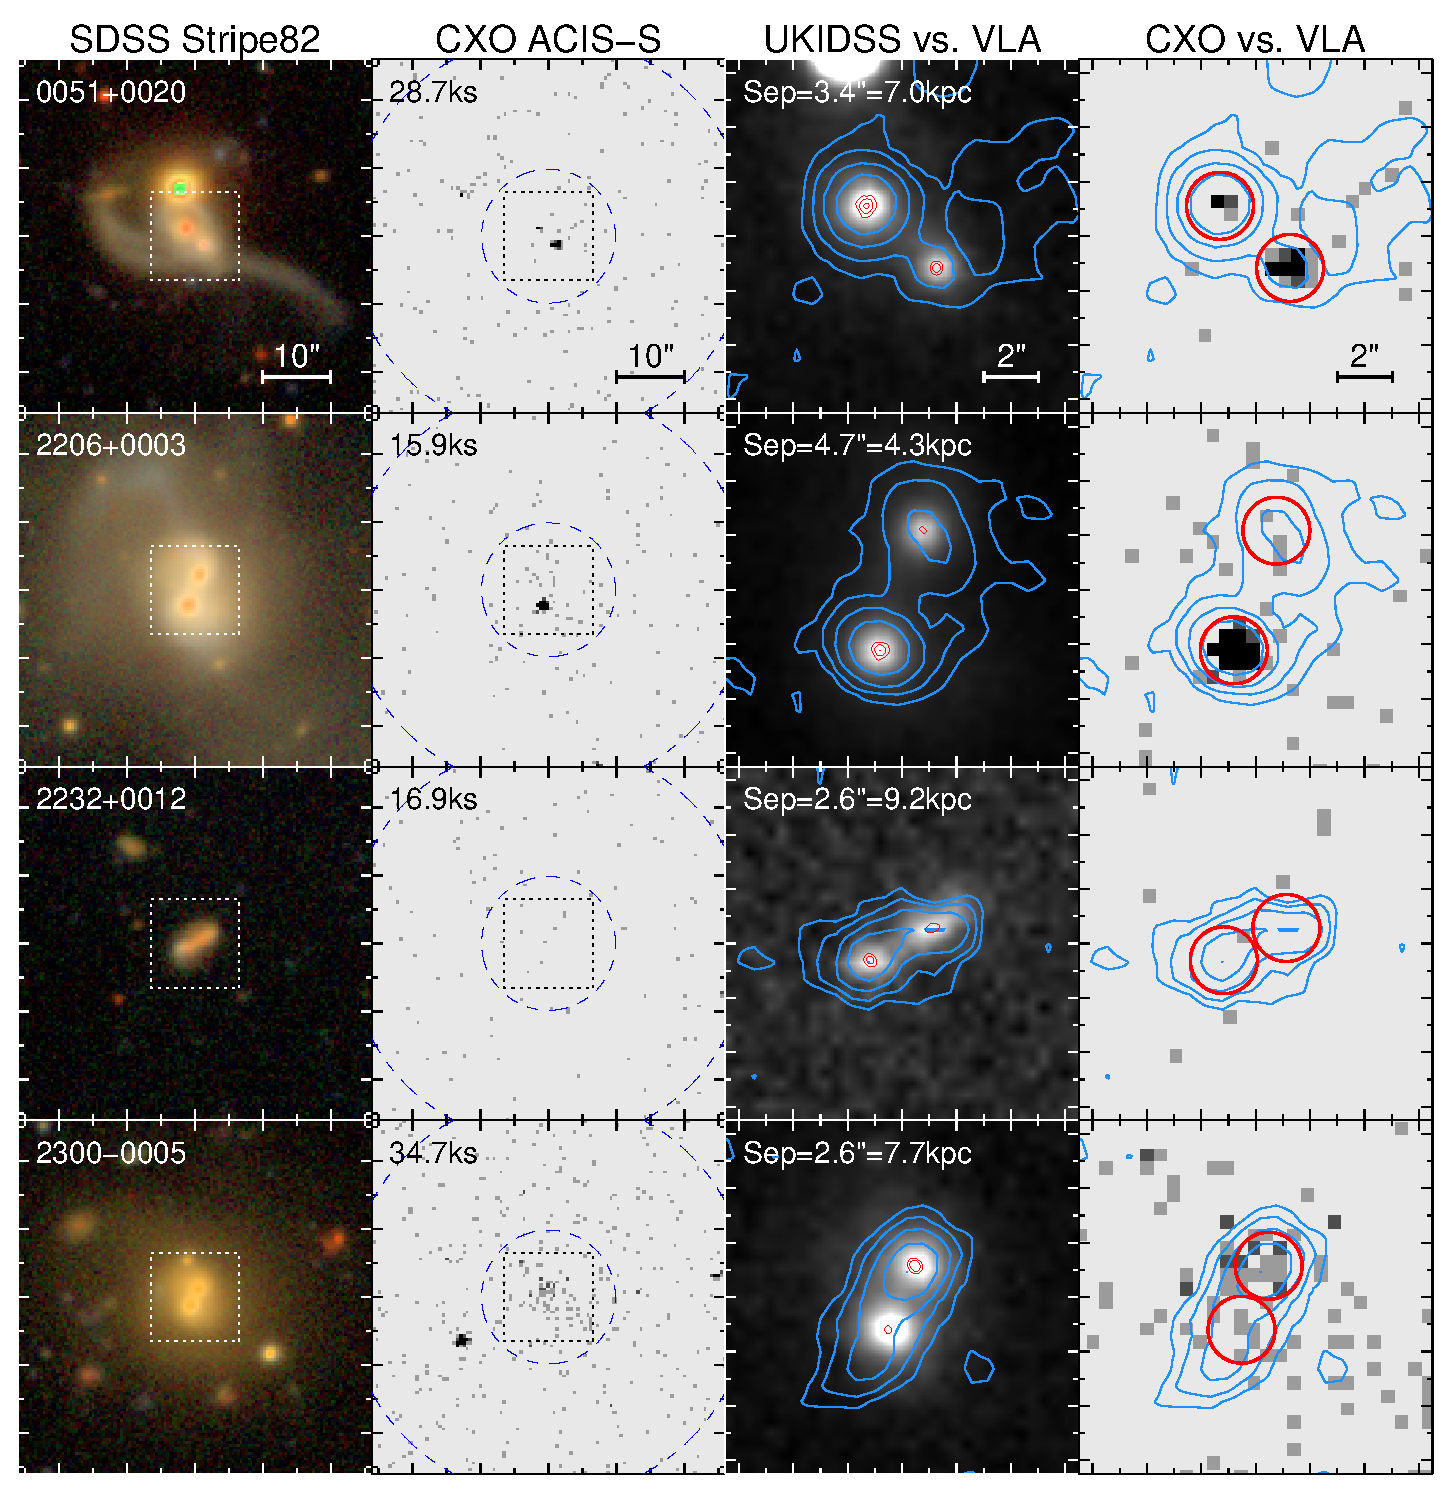
\includegraphics[width=0.95\linewidth]{figs/showxray.eps}
\caption{Optical, near-IR, and X-ray images of the dual AGNs, with radio contours. For each system, we show from left to right: the wide-field SDSS deep-coadded $gri$ color image, the wide-field ACIS image, a narrow-field UKIDSS $J$-band image overlaid with the VLA 6\,GHz map ({\it red} contours; 0.3\arcsec\ beam) and the 1.4\,GHz map from the VLA-Stripe82 survey ({\it blue} contours; 1.\arcsec8\ beam), and the narrow-field ACIS image overlaid with the 1.4\,GHz map. The X-ray images are not smoothed and are displayed in their native $\sim$0.\arcsec5\ pixels. The dotted squares in the wide-field images show the area covered by the narrow-field images. The annulus region used to estimate the X-ray background is shown as blue dashed circles in the second column and the source apertures are shown as red circles in the last column. The 6\,GHz VLA contours are at ($+$3, $+$6, $+$24, $+$96)$\times$$\sigma$. The 1.4\,GHz VLA contours start at 2$\sigma$ and the levels increase exponentially to the peak S/N. Major tickmarks are spaced in 10\arcsec\ intervals in the wide-field columns and 2\arcsec\ intervals in the narrow-field columns. The short designation, the \chandra\ exposure time, and the projected separation of the 6\,GHz radio cores are labeled. N is up and E is left for all panels. 
\label{fig:xrayimgs}}
\end{figure*}

Our sample consists of four radio-selected kpc-scale dual AGNs at $0.04 < \rm z < 0.22$ in the SDSS Stripe 82 field  \citepalias{Fu15b}. The four galaxy pairs have projected angular separations between 2.5\arcsec\ and 4.6\arcsec\ and all of the eight nuclei show compact radio emission at a resolution of 0.\arcsec3. Under \chandra\ Cycle 18 Proposal \# 18700044 (PI: H. Fu), we observed the targets with the Advanced CCD Imaging Spectrometer (ACIS) in October 2016 (Obs ID: 19456) and September 2017 (Obs IDs: 19453-19455). The targets were placed near the aim point on the back-illuminated S3 chip. The average integration time is 24\,ks. 

Data reduction and analysis is carried out with the \chandra\ Interactive Analysis of Observations software \citep[CIAO v4.9;][]{Fruscione06}. Because the first observation and the last observation took place almost a year apart, we reprocess all of the data to the calibration database (CALDB v4.7.7) with \texttt{chandra\_repro}. We then focus on the data of the S3 chip (CCD ID: 7) in the calibrated energy range between 0.3 and 10\,keV by filtering the calibrated level 2 event file with \texttt{dmcopy}. Only the events with grades 0, 2, 3, 4, and 6 were included. We detect no significant flares in the background light curves. In the observation of 2206$+$0003, the X-ray position of the southeast component of the binary (i.e., 2206$+$0003\,SE) shows an offset of 0.26\arcsec\ from the VLA 6\,GHz source. We correct for this astrometric offset in the ASOL file and the event-2 file with \texttt{wcs\_update}. The other three observations show no significant astrometric offset wherever there are sufficient number of X-ray sources to carry out a positional comparison between the X-ray sources from \texttt{wavdetect} and the radio sources from our VLA observations and the near-infrared sources from UKIDSS. 

Figure\,\ref{fig:xrayimgs} shows the full-band (0.3-8 keV) X-ray images of the targets, along with the deep coadded optical images from the SDSS \citep{Jiang14}, near-IR images from UKIRT Infrared Deep Sky Survey \citep[UKIDSS;][]{Warren07}, and radio contours from the VLA Stripe 82 1.4\,GHz observations \citep[VS82;][]{Hodge11} and our VLA 6\,GHz observations (\citetalias{Fu15b}). The first impression of the figure is that four of the eight nuclei are clearly detected (0051$+$0020\,NE, 0051$+$0020\,SW, 2206$+$0003\,SE, and 2300$-$0005\,NW), two are probably detected (2206$+$0003\,NW and 2300$-$0005\,SE), and two are clearly undetected (2232$+$0012\,NW and 2232$+$0012\,SE). We present more quantitative results from aperture photometry in the next section.

\section{X-ray Data Analysis} \label{sec:analysis}

\subsection{Photometry} \label{sec:photo}

For source photometry, we adopt a 2.5\,pixel-radius circular aperture centered at the VLA 6\,GHz position (the native CCD pixel size of ACIS-S is 0\farcs4920). The source aperture encloses 92\%/88\% of the PSF at an effective energy of 1.5/3.6\,keV from \texttt{arfcorr} and its diameter of 2\farcs46 is slightly less than the angular separation of the most closely separated pair in our sample (thus avoiding aperture overlapping). The aperture is also large enough to fully enclose the 90\% ACIS-S positional uncertainty radius of $\sim$0.7\arcsec\ (\url{http://cxc.harvard.edu/cal/ASPECT/celmon/}). To estimate the background contribution to the source counts, we define a background region using an annulus centered at the middle point of each pair with an inner and an outer radius of 20 pixels and 60 pixels, respectively. We exclude sources detected by \texttt{wavdetect} inside the background annulus with a 10\,pixel-radius circular region around each source. Counts from the source and background regions are measured with \texttt{srcflux} for three energy bands: soft ($S$; 0.3$-$2\,keV, $E_{\rm eff} = 1.5$\,keV), hard ($H$; 2$-$8\,keV, $E_{\rm eff} = 4.3$\,keV), and full ($F$; 0.3$-$8\,keV, $E_{\rm eff} = 3.6$\,keV), where the effective energy ($E_{\rm eff}$) is defined as the effective-area-weighted mean energy of each band. The full-band source counts range between 0 and 72, whereas the background is expected to contribute between 0.2 and 0.6 counts in the source aperture. The significance of the X-ray detections can be estimated using Poisson statistics. The probability of obtaining the observed counts or more in the source aperture from background events can be calculated using the cumulative probability distribution function of the Poisson distribution:
\begin{equation} \label{eq:significance}
P(\geq k | \lambda; {\rm no\,source}) = \sum_{m=k}^{\infty} \frac{\lambda^m e^{-\lambda}}{m!} = 1-\sum_{m=0}^{k-1} \frac{\lambda^m e^{-\lambda}}{m!}
\end{equation}
where $k$ and $\lambda$ are the observed counts and the expected background counts in the source aperture, respectively. For the six AGNs in 0051$+$0020, 2206$+$0003, and 2300$-$0005, this ``no-source'' probability is less than 0.1\% in the 0.3$-$8\,keV band, which is equivalent to a confidence level of $>$99.9\% for a detection of the source. We thus consider these six sources as robust detections. Both AGNs in 2232$+$0012 are undetected, so we estimate the 3$\sigma$ (99\%) upper limits of the count rates using the background-marginalized Bayesian algorithm built into \texttt{aprates} and convert them to flux upper limits assuming an unabsorbed power law model with $\Gamma = 1.9$, which is appropriate for AGNs \citep[e.g.,][]{Just07,She17}. The statistical results are consistent with the visual impression of Fig.~\ref{fig:xrayimgs}. The total counts and the expected background counts in the three energy bands are listed in Table\,\ref{tab:xraydata}, along with a few derived parameters discussed below.

We estimate the hardness ratio, HR\,$\equiv (H-S)/(H+S)$, of the six detections using the Bayesian estimation method of \citet{Park06}. Assuming an intrinsic power-law spectrum with a fixed photon index, we can use the estimated HR to infer the intervening total Hydrogen column density in the host galaxy ($N_{\rm H}$). We again adopt the canonical power-law photon index of $\Gamma = 1.9$. For each target, we use the \texttt{modelflux} task to calculate the relation between HR and $N_{\rm H}$ for a redshifted power-law model with $\Gamma = 1.9$ absorbed intrinsically by the torus or the host galaxy and subsequently by $N_{\rm H}^{\rm Gal}$ from the Milky Way (\texttt{xszpowerlw * xszphabs * xsphabs}). The photoelectric absorption cross-sections \citep{Morrison83} assume the standard Solar abundance set from \citet{Anders89}. The HR$-$$N_{\rm H}$ relation varies among the sources because of the differences in redshift, the Galactic column density ($N_{\rm H}^{\rm Gal}$), and the Auxiliary Response Function (ARF) and Redistribution Matrix Function (RMF) specific to the \chandra\ observation. The Galactic column densities from the NRAO catalog \citep{Dickey90} range between $2.66\times10^{20}$\,cm$^{-2}$ and $5.21\times10^{20}$\,cm$^{-2}$. 

We can apply the HR-based method to self-consistently convert the count rate to fluxes for three of the six detections (both sources in 0051$+$0020 and 2206$+$0003SE), because they have HRs greater than the unabsorbed power-law model (i.e., ${\rm HR} > -0.4$). We first use the HR$-$$N_{\rm H}$-relation and the measured HR to estimate $N_{\rm H}$ and we obtain $10^{21}$\,cm$^{-2} \lesssim N_{\rm H} \lesssim 5\times10^{22}$\,cm$^{-2}$. We then scale the PSF-corrected count rate to the absorbed and the unabsorbed flux in each energy band using the scaling factors from \texttt{modelflux} for the HR-derived $N_{\rm H}$. The X-ray emission from these three sources appears spatially concentrated on the radio positions in Fig.\,\ref{fig:xrayimgs} (as expected from point sources) and their HRs are consistent with nuclear emission typically observed in AGNs. Therefore, we conclude that the X-ray emission in 0051$+$0020 and 2206$+$0003SE are powered by BH accretion and one of the three AGNs are obscured ($N_{\rm H} > 10^{22}$\,cm$^{-2}$).

The HRs of the other three detections (2206$+$0003NW, and both sources in 2300$-$0005) are lower than the HR of an unabsorbed power-law model (${\rm HR} < -0.4$), so we calculate their fluxes by setting $N_{\rm H} = 0$. The low HRs of these three sources imply intrinsically softer spectra, likely dominated by diffuse kpc-scale nonnuclear thermal plasma with $T \sim 10^7$\,K (i.e., $kT \sim 1$\,keV) in the host galaxies \citep[e.g.,][]{Donato04}. For reference, the intrinsic HR is about $-0.8$ for an \texttt{apec} thermal plasma model with $kT = 1$\,keV and $Z = 0.2\,Z_\odot$. The X-ray emission of these sources appears spatially extended in Fig.\,\ref{fig:xrayimgs}, but their counts are too low to allow a measurement of the angular sizes or a spatial decomposition between the host galaxy and the central point source. Therefore, the X-ray fluxes in 2206$+$0003NW and 2300$-$0005 should be considered as strict upper limits of nuclear X-ray emission from AGNs.

\begin{deluxetable*}{lcccrccccc}
\tabletypesize{\small} % \normalsize \small \footnotesize \scriptsize
\tablewidth{0pt}
\tablecaption{X-ray Observations and Photometry 
\label{tab:xraydata}}
\tablehead{ 
\colhead{Object} & \colhead{Radio Designation} & \colhead{Exptime} & \colhead{Full} & \colhead{Soft} & \colhead{Hard} & \colhead{HR} & \colhead{$\log N_{\rm H}$} & \colhead{$\log F_{\rm 0.3-8keV}^{\rm abs}$} & \colhead{$\log F_{\rm 0.3-8keV}^{\rm unabs}$} \\ 
\colhead{} & \colhead{(J2000)} & \colhead{(ks)} & \colhead{src (bkg)} & \colhead{src (bkg)} & \colhead{src (bkg)} & \colhead{} & \colhead{(cm$^{-2}$)} & \colhead{(erg~s$^{-1}$~cm$^{-2}$)} & \colhead{(erg~s$^{-1}$~cm$^{-2}$)} \\ 
\colhead{(1)} & \colhead{(2)} & \colhead{(3)} & \colhead{(4)} & \colhead{(5)} & \colhead{(6)} & \colhead{(7)} &  \colhead{(8)} & \colhead{(9)} & \colhead{(10)}
}
\startdata 
%0051$+$0020SW&005113.93$+$002047.2&28.7&30 (0.3)&19 (0.1)&11 (0.2)&$-0.28_{-0.17}^{+0.18}$&$21.23_{-1.23}^{+0.51}$&$-13.89_{-0.08}^{+0.08}$&$-13.75_{-0.15}^{+0.19}$\\
0051$+$0020NE&005114.11$+$002049.5&28.7& 6 (0.3)& 3 (0.1)& 3 (0.2)&$-0.02_{-0.40}^{+0.40}$&$21.89_{-1.89}^{+0.45}$&$-14.56_{-0.21}^{+0.17}$&$-14.30_{-0.44}^{+0.39}$\\
2206$+$0003NW&220634.98$+$000327.6&15.9& 3 (0.2)& 2 (0.1)& 1 (0.1)&$-0.63_{-0.26}^{+0.53}$&                  \nod &$-14.63_{-0.31}^{+0.25}$&$-14.57_{-0.31}^{+0.25}$\\
2206$+$0003SE&220635.08$+$000323.2&15.9&72 (0.2)& 7 (0.1)&65 (0.1)&$+0.82_{-0.08}^{+0.06}$&$22.71_{-0.09}^{+0.09}$&$-12.95_{-0.05}^{+0.05}$&$-12.44_{-0.11}^{+0.11}$\\
2232$+$0012NW&223222.44$+$001225.9&16.9& 0 (0.2)& 0 (0.1)& 0 (0.1)&                  \nod &                  \nod &               $<-14.44$& $<-14.38$\\
2232$+$0012SE&223222.60$+$001224.7&16.9& 1 (0.2)& 0 (0.1)& 1 (0.1)&                  \nod &                  \nod &               $<-14.29$& $<-14.23$\\
2300$-$0005NW&230010.18$-$000531.6&34.7&12 (0.6)&10 (0.3)& 2 (0.3)&$-0.78_{-0.17}^{+0.23}$&                  \nod &$-14.39_{-0.14}^{+0.12}$&$-14.34_{-0.14}^{+0.12}$\\
2300$-$0005SE&230010.24$-$000533.9&34.7& 6 (0.6)& 4 (0.3)& 2 (0.3)&$-0.47_{-0.35}^{+0.42}$&                  \nod &$-14.72_{-0.22}^{+0.18}$&$-14.66_{-0.22}^{+0.18}$\\

0051$+$0020SW&005113.93$+$002047.2&28.7&30 (0.3)&19 (0.1)&11 (0.2)&$-0.28_{-0.17}^{+0.18}$&$21.23_{-1.23}^{+0.51}$&$-13.89_{-0.08}^{+0.08}$&$-13.75_{-0.15}^{+0.19}$\\
0051$+$0020NE&005114.11$+$002049.5&28.7& 6 (0.3)& 3 (0.1)& 3 (0.2)&$-0.02_{-0.40}^{+0.40}$&$21.89_{-1.89}^{+0.45}$&$-14.56_{-0.21}^{+0.17}$&$-14.30_{-0.44}^{+0.39}$\\
\\
2206$+$0003NW&220634.98$+$000327.6&15.9& 3 (0.2)& 2 (0.1)& 1 (0.1)&$-0.63_{-0.26}^{+0.53}$&                  \nod &$-14.63_{-0.31}^{+0.25}$&$-14.57_{-0.31}^{+0.25}$\\
2206$+$0003SE&220635.08$+$000323.2&15.9&72 (0.2)& 7 (0.1)&65 (0.1)&$+0.82_{-0.08}^{+0.06}$&$22.71_{-0.09}^{+0.09}$&$-12.95_{-0.05}^{+0.05}$&$-12.44_{-0.11}^{+0.11}$\\
\\
2232$+$0012NW&223222.44$+$001225.9&16.9& 0 (0.2)& 0 (0.1)& 0 (0.1)&                  \nod &                  \nod &               $<-14.44$& $<-14.38$\\
2232$+$0012SE&223222.60$+$001224.7&16.9& 1 (0.2)& 0 (0.1)& 1 (0.1)&                  \nod &                  \nod &               $<-14.29$& $<-14.23$\\
\\
2300$-$0005NW&230010.18$-$000531.6&34.7&12 (0.6)&10 (0.3)& 2 (0.3)&$-0.78_{-0.17}^{+0.23}$&                  \nod &$-14.39_{-0.14}^{+0.12}$&$-14.34_{-0.14}^{+0.12}$\\
2300$-$0005SE&230010.24$-$000533.9&34.7& 6 (0.6)& 4 (0.3)& 2 (0.3)&$-0.47_{-0.35}^{+0.42}$&                  \nod &$-14.72_{-0.22}^{+0.18}$&$-14.66_{-0.22}^{+0.18}$\\

\enddata
\tablecomments{ 
Rows are grouped in sets of two that each include a pair, and sources are sorted in ascending R.A.
(1) Object name.
(2) J2000 coordinates of the radio cores from our 0.3\arcsec\ VLA 6\,GHz images \citepalias{Fu15b}.
(3) ACIS-S exposure time in kilosecond.
(4$-$6) source and background counts inside a 2.5\arcsec-diameter circular aperture centered on the radio position for full band ($F$, 0.3$-$8\,keV), soft band ($S$, 0.3$-$2.0\,keV), and hard band ($H$, 2.0--8.0\,keV), respectively.
(7) Hardness ratio (HR) determined using Bayesian estimation method \citep[BEHR;][]{Park06}, which is defined as HR\,$=(H-S)/(H+S)$; quoted are the mode and the 15.8-and-84.1-percentiles.
(8) Intrinsic hydrogen column density inferred from HR by fixing the photon index at $\Gamma = 1.9$. Three of the six detected sources do not have $N_{\rm H}$ measurements because their nominal HRs are softer than the assumed power-law.
(9$-$10) Absorbed and unabsorbed power-law model flux at the observed-frame full band. The absorbed flux includes both intrinsic absorption and Galactic absorption. Detections are quoted with the 1$\sigma$ uncertainty, and non-detections are listed as upper limits at 99\% confidence level. The quoted error of the unabsorbed flux accounts for the uncertainties in both the count rate and the HR-derived intrinsic column density.
}
\end{deluxetable*}

\subsection{Spectral Fitting} \label{sec:spec_fit}

Given the limited counts, spectral fitting is only possible for 2206$+$0003\,SE, which has 72 counts. We extracted the spectrum between 0.3 and 8\,keV using \texttt{specextract} with the same aperture as used in our aperture photometry. Using \texttt{Sherpa}, we group the spectrum to a minimum of 5 counts per bin and fit the grouped spectrum using $\chi^{2}$ statistics and the Levenberg-Marquart optimization method. The assumed spectral model consists of a power law attenuated by Galactic absorption (fixed at $\log N_{\rm H}^{\rm Gal} = 4.64\times10^{20}$\,cm$^{-2}$) as well as intrinsic absorption at the redshift of the source. Because the data is insufficient to constrain both the power-law photon index ($\Gamma$) and the intrinsic column density ($\log N_{\rm H}$), we fix the former to the canonical value of $\Gamma = 1.9$. The best-fit model is plotted against the grouped spectrum in Fig.~\ref{fig:sherpa}. The best-fit model has a $\chi^2$ residual of 8.6 for a degree-of-freedom (dof) of 12. The best-fit value and 1$\sigma$ uncertainty for the intrinsic column density is $\log N_{\rm H} = 23.09^{+0.15}_{-0.16}$\,cm$^{-2}$. The column density is 0.4\,dex higher than that inferred from the hardness ratio in Table\,\ref{tab:xraydata}, $\log N_{\rm H} = 22.70\pm0.09$\,cm$^{-2}$, confirming that 2206$+$0003\,SE is a moderately absorbed source. Because the $\chi^2$ of the spectral fit is mostly determined by the data points above 2\,keV, the HR of the best-fit spectral model ($\simeq$ 0.95) is significantly higher than the observed HR of 0.82, explaining why the column density is overestimated by $\sim0.4$\,dex. For this reason, we quote the HR-derived column density in this paper. 

\begin{figure}
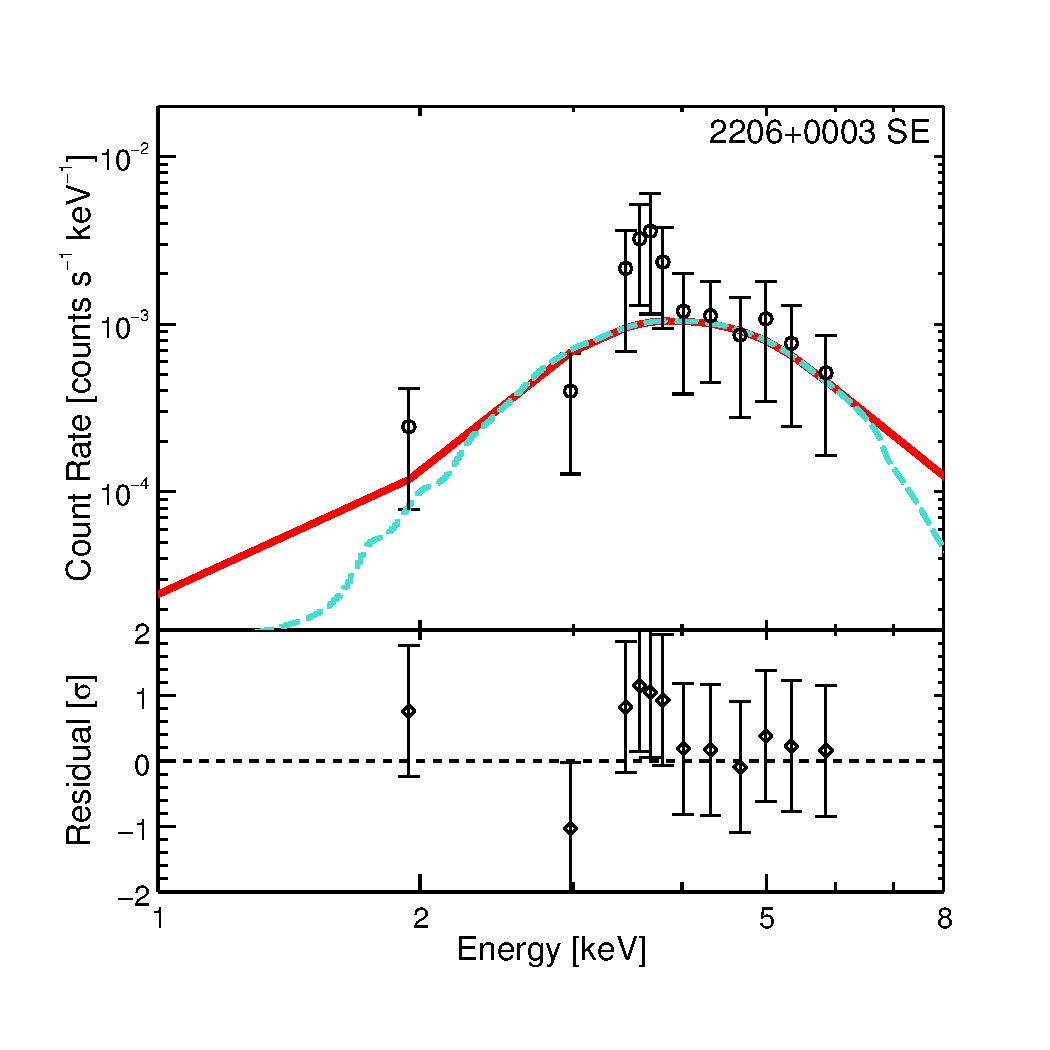
\includegraphics[width=8.5cm]{figs/spectral_fit_PLf.pdf}
\caption{\chandra\ ACIS spectrum of 2206$+$0003SE. The red solid curve shows the best-fit absorbed power-law model with energy bins matched to the data, while the turquoise dashed curve is the super-resolution model with 0.1\,keV bins. The lower panel shows the residuals of the best-fit model in units of $\sigma$, the Poisson uncertainty of the counts in each bin. The sharp decline of soft X-ray counts below $\sim$3\,keV indicates heavy obscuration ($N_{\rm H} > 10^{22}$\,cm$^{-2}$) by intervening gas in a circumnuclear torus and/or the ISM of the host galaxy. The nature of the emission feature at $\sim$3.8\,keV is unclear.}
\label{fig:sherpa}
\end{figure}

Although the absorbed power-law model is already a good fit to the data, there appears to be a narrow emission feature centered near $\sim$3.8\,keV that is not captured by the model. We attempt fitting this feature by adding a Gaussian component to the power-law model. The reduced statistic for this more complex model is $\chi^{2}/{\rm dof} = 4.35/9$. The best-fit Gaussian is centered at rest-frame $3.8\pm0.1$\,keV and has a width of $\sigma = 130^{+150}_{-90}$\,eV. Note that the best-fit line width is consistent with being unresolved at $<$2$\sigma$ confidence level, even though the nominal value appears wider than the ACIS-S3 energy resolution ($\sigma \sim 64$\,eV at 5.9\,keV; \href{http://cxc.harvard.edu/proposer/POG/html/chap6.html#tth_sEc6.7}{The Chandra Proposers' Observatory Guide}). 
An F-test suggests that a more complex model containing a Gaussian to account for the emission feature does not significantly improve the fit, and so we default to the simpler model without a Guassian in Fig.~\ref{fig:sherpa}.
\begin{comment}
To check whether introducing the additional model parameters is statistically warranted, we conduct an $F$-test of the two spectral models. As usual, the $F$-ratio is defined as:
\begin{equation}
F = \frac{(\chi^2_1-\chi^2_2)/(p_2-p_1)}{\chi^2_2/(N-p_2)}
\end{equation}
where the subscripts 1 and 2 denote the simpler model and the complex model, respectively, $p$ is the number of free parameters, and $N$ is the number of data points. For our case, we obtain an $F$-ratio of 2.93 for $\chi^2_1 = 8.6, \chi^2_2 = 4.35, p_1 = 2, p_2 = 5$, and $N = 14$. Following the $F$ distribution with $(p_2-p_1, N-p_2)$ degrees of freedom, the probability that a random $F$-ratio is greater than the observed value of 2.93 is 9.2\%, indicating that the simpler model can only be rejected at a rather high false-rejection probability of 9.2\% (which is typically set to 1\%). Thus we conclude that the more complex model does not provide a significantly better fit the data. Deeper X-ray data are clearly needed to verify or refute the existence of this unidentified narrow emission feature.
\end{comment}

\section{Results} \label{sec:results}

Our \chandra\ observations provide the X-ray fluxes and the HRs of our dAGNs, and for several cases, the column densities of the intervening gas (Table\,\ref{tab:xraydata}). To estimate the unabsorbed X-ray luminosity at rest-frame 2$-$10\,keV ($L_{\rm X} \equiv L_{\rm 2-10 keV}$), we use the $K$-correction factor of the assumed power-law model to convert the unabsorbed 0.3$-$8\,keV flux to the rest-frame flux in 2$-$10\,keV.
%
For the range of column densities observed in our sources ($N_{\rm H} < 10^{23}$\,cm$^{-2}$), the 2$-$10\,keV luminosity is almost unaffected by absorption: photoelectric absorption by intervening gas with $N_{\rm H} = 10^{23}$\,cm$^{-2}$ only decreases the 2-10\,keV luminosity by 0.28\,dex. 

In Table\,\ref{tab:luminosity}, we list the X-ray luminosity along with other multi-wavelength properties for individual dAGN components. Below we briefly summarize the observed properties of the sample from \citetalias{Fu15a} and \citetalias{Fu15b}: 

\begin{enumerate}

\item Four sources in two dAGNs (2232$+$0012 and 2300$-$0005) show significant excess in 1.4\,GHz radio luminosity compared to their H$\alpha$ luminosity. Such a radio excess indicates the existence of an additional radio-emitting component besides the synchrotron emission from cosmic rays accelerated by star formation. Most likely this additional component is a radio-loud AGN. 

\item The remaining four sources in 0051$+$0020 and 2206$+$0003 do not show significant radio excess, although they show systematically higher radio luminosity for their H$\alpha$ luminosity when compared to the radio-detected star-forming galaxies in the same field. They are classified as AGNs because their optical emission-line ratios fall in either the AGN-starforming composite region or the LINER region on the [O\,{\sc iii}]/H$\beta$ vs. [N\,{\sc ii}]/H$\alpha$ BPT diagram. None of these four galaxies are retired galaxies whose emission lines are powered by post-AGB stars because their H$\alpha$ EW well exceeds the threshold value at 3\,\AA. 

\item Half of the radio-excess AGNs are high-excitation radio galaxies (HERGs) and half are low-excitation radio galaxies \citep[LERGs;][]{Laing94}. Both AGNs in 2232$+$0012 are HERGs, with [O\,{\sc iii}]/H$\alpha > 0.2$, EW$_{\rm [O\,III]} > 3$\,\AA, and BPT classifications of composite galaxies. And both AGNs in 2300$-$0005 are LERGs with no detectable emission lines. 

\item All of the sources show compact ($\lesssim$0.4\arcsec), sub-mJy ($0.07 < S_{\rm 6GHz} < 0.93$\,mJy) radio emission centered on the nuclei in our $C$-band 0.3\arcsec-resolution VLA observations. Only 2300$-$0005NW shows a nearly flat spectrum within the $C$-band frequency range ($\alpha \simeq 0.5$ between 4 and 8\,GHz); the rest show much steeper spectra in the same frequency range ($0.9 < \alpha < 1.8$).

\item The rest-frame 5\,GHz luminosity of the radio cores range between $37.3 < $ log$\,L_{\rm 5GHz}/{\rm erg~s}^{-1} < 39.4$, which is also comparable with nearby LLAGNs and Seyferts \citep{Ho08,She17}.

\item Based on the SDSS and Keck optical spectra, we measure stellar velocity dispersions between $110 < \sigma_\star < 320$\,\kms, which imply BH masses between $7.4 < \log(M_{\rm BH}) < 9.4$ using the $M_{\rm BH}-\sigma_\star$ relation of nearby classical bulges and elliptical galaxies \citep{Kormendy13}. 

\end{enumerate}

In the following sub-sections, we perform a series of comparisons between the dAGNs and the general AGN population. We begin by comparing the general AGN properties such as radio-to-X-ray ratio, Eddington ratio, and the BH fundamental plane in \S~\ref{sec:Lx}. We then compare the distribution of X-ray hardness ratios in \S~\ref{sec:HR} to test whether the AGNs in mergers are more obscured than isolated AGNs because of tidally induced inflows. Finally, in \S~\ref{sec:deficit} we check if the X-ray luminosities of dAGNs are lower than expected from their mid-IR and [O\,{\sc iii}] luminosities and discuss the role of star formation in the dAGNs. 

\begin{deluxetable*}{lcccccccc}
\tabletypesize{\small} % \normalsize \small \footnotesize \scriptsize
\tablewidth{0pt}
\tablecaption{Multi-Wavelength Properties
\label{tab:luminosity}}
\tablehead{ 
\colhead{Object} & \colhead{$z$} & \colhead{$\sigma_{\star}$} & \colhead{$\log M_{\rm BH}$} & \colhead{$\log L_{\rm H\alpha}$} & \colhead{$\log L_{\rm [OIII]}$} & \colhead{$\log L_{\rm 5GHz}$} & \colhead{$\log L_{\rm 12\mu m}$} & \colhead{$\log L_{\rm X}$} \\
\colhead{} & \colhead{} & \colhead{(km~s$^{-1}$)} & \colhead{(\msun)} & \colhead{(erg~s$^{-1}$)} & \colhead{(erg~s$^{-1}$)} & \colhead{(erg~s$^{-1}$)} & \colhead{(erg~s$^{-1}$)} & \colhead{(erg~s$^{-1}$)} \\
\colhead{(1)} & \colhead{(2)} & \colhead{(3)} & \colhead{(4)} & \colhead{(5)} & \colhead{(6)} & \colhead{(7)} &  \colhead{(8)} & \colhead{(9)} 
}
\startdata 
%0051$+$0020SW&0.11253&$140\pm12$&$7.8\pm0.3$&$41.80\pm0.02$&$41.33\pm0.11$&$38.73\pm0.02$&$43.88\pm0.02$&$41.49_{-0.15}^{+0.19}$\\
0051$+$0020NE&0.11257&$166\pm 9$&$8.1\pm0.3$&$42.36\pm0.01$&$41.37\pm0.18$&$39.22\pm0.01$&\nodata       &$40.95_{-0.44}^{+0.39}$\\
2206$+$0003NW&0.04656&$114\pm 9$&$7.4\pm0.3$&$41.23\pm0.01$&$40.63\pm0.06$&$37.37\pm0.10$&$42.77\pm0.02$&$39.87_{-0.31}^{+0.25}$\\
2206$+$0003SE&0.04640&$170\pm 6$&$8.2\pm0.3$&$41.55\pm0.01$&$41.20\pm0.03$&$38.22\pm0.01$&\nodata       &$41.99_{-0.11}^{+0.11}$\\
2232$+$0012NW&0.22128&$244\pm36$&$8.9\pm0.4$&$41.18\pm0.04$&$40.47\pm0.08$&$39.03\pm0.04$&$44.17\pm0.02$&               $<$41.51\\
2232$+$0012SE&0.22187&$210\pm61$&$8.6\pm0.6$&$41.51\pm0.04$&$41.15\pm0.08$&$39.28\pm0.02$&\nodata       &               $<$41.66\\
2300$-$0005NW&0.17971&$284\pm13$&$9.2\pm0.3$&      $<$40.50&      $<$40.05&$39.40\pm0.01$&$43.28\pm0.17$&$41.35_{-0.14}^{+0.12}$\\
2300$-$0005SE&0.17981&$324\pm11$&$9.4\pm0.3$&      $<$40.62&      $<$40.12&$38.52\pm0.09$&\nodata       &$41.03_{-0.22}^{+0.18}$\\

0051$+$0020SW&0.11253&$140\pm12$&$7.8\pm0.3$&$41.80\pm0.02$&$41.33\pm0.11$&$38.73\pm0.02$&$43.88\pm0.02$&$41.49_{-0.15}^{+0.19}$\\
0051$+$0020NE&0.11257&$166\pm 9$&$8.1\pm0.3$&$42.36\pm0.01$&$41.37\pm0.18$&$39.22\pm0.01$&\nodata       &$40.95_{-0.44}^{+0.39}$\\
\\
2206$+$0003NW&0.04656&$114\pm 9$&$7.4\pm0.3$&$41.23\pm0.01$&$40.63\pm0.06$&$37.37\pm0.10$&$42.77\pm0.02$&$39.87_{-0.31}^{+0.25}$\\
2206$+$0003SE&0.04640&$170\pm 6$&$8.2\pm0.3$&$41.55\pm0.01$&$41.20\pm0.03$&$38.22\pm0.01$&\nodata       &$41.99_{-0.11}^{+0.11}$\\
\\
2232$+$0012NW&0.22128&$244\pm36$&$8.9\pm0.4$&$41.18\pm0.04$&$40.47\pm0.08$&$39.03\pm0.04$&$44.17\pm0.02$&               $<$41.51\\
2232$+$0012SE&0.22187&$210\pm61$&$8.6\pm0.6$&$41.51\pm0.04$&$41.15\pm0.08$&$39.28\pm0.02$&\nodata       &               $<$41.66\\
\\
2300$-$0005NW&0.17971&$284\pm13$&$9.2\pm0.3$&      $<$40.50&      $<$40.05&$39.40\pm0.01$&$43.28\pm0.17$&$41.35_{-0.14}^{+0.12}$\\
2300$-$0005SE&0.17981&$324\pm11$&$9.4\pm0.3$&      $<$40.62&      $<$40.12&$38.52\pm0.09$&\nodata       &$41.03_{-0.22}^{+0.18}$\\

\enddata
\tablecomments{ 
(1) Object name;
(2-3) spectroscopic redshift and stellar velocity dispersion from fitting SDSS and Keck/LRIS spectra with stellar population synthesis models \citepalias{Fu15b};
(4) black hole mass inferred from the $M_{\rm BH}-\sigma_\star$ relation of \citet{Kormendy13}, which has an intrinsic scatter of $\sim$0.29\,dex;
(5-6) H$\alpha$ and [O\,{\sc iii}]\,$\lambda$5007 line luminosities, corrected for reddening and aperture-loss;
(7) rest-frame 5\,GHz luminosity ($\nu L_{\nu}$) computed from the VLA flux density at 6\,GHz \citepalias{Fu15b};
(8) rest-frame 12\,\um\ luminosity from AllWISE photometry (listed is the total luminosity for each pair because the components are blended in WISE images);
(9) unabsorbed rest-frame 2-10\,keV luminosity $K$-corrected from the unabsorbed model flux ($F_{\rm 0.3-8keV}^{\rm unabs}$) in Table\,\ref{tab:xraydata}.
%
}
\end{deluxetable*}

\subsection{General AGN properties} \label{sec:Lx}

\begin{figure}
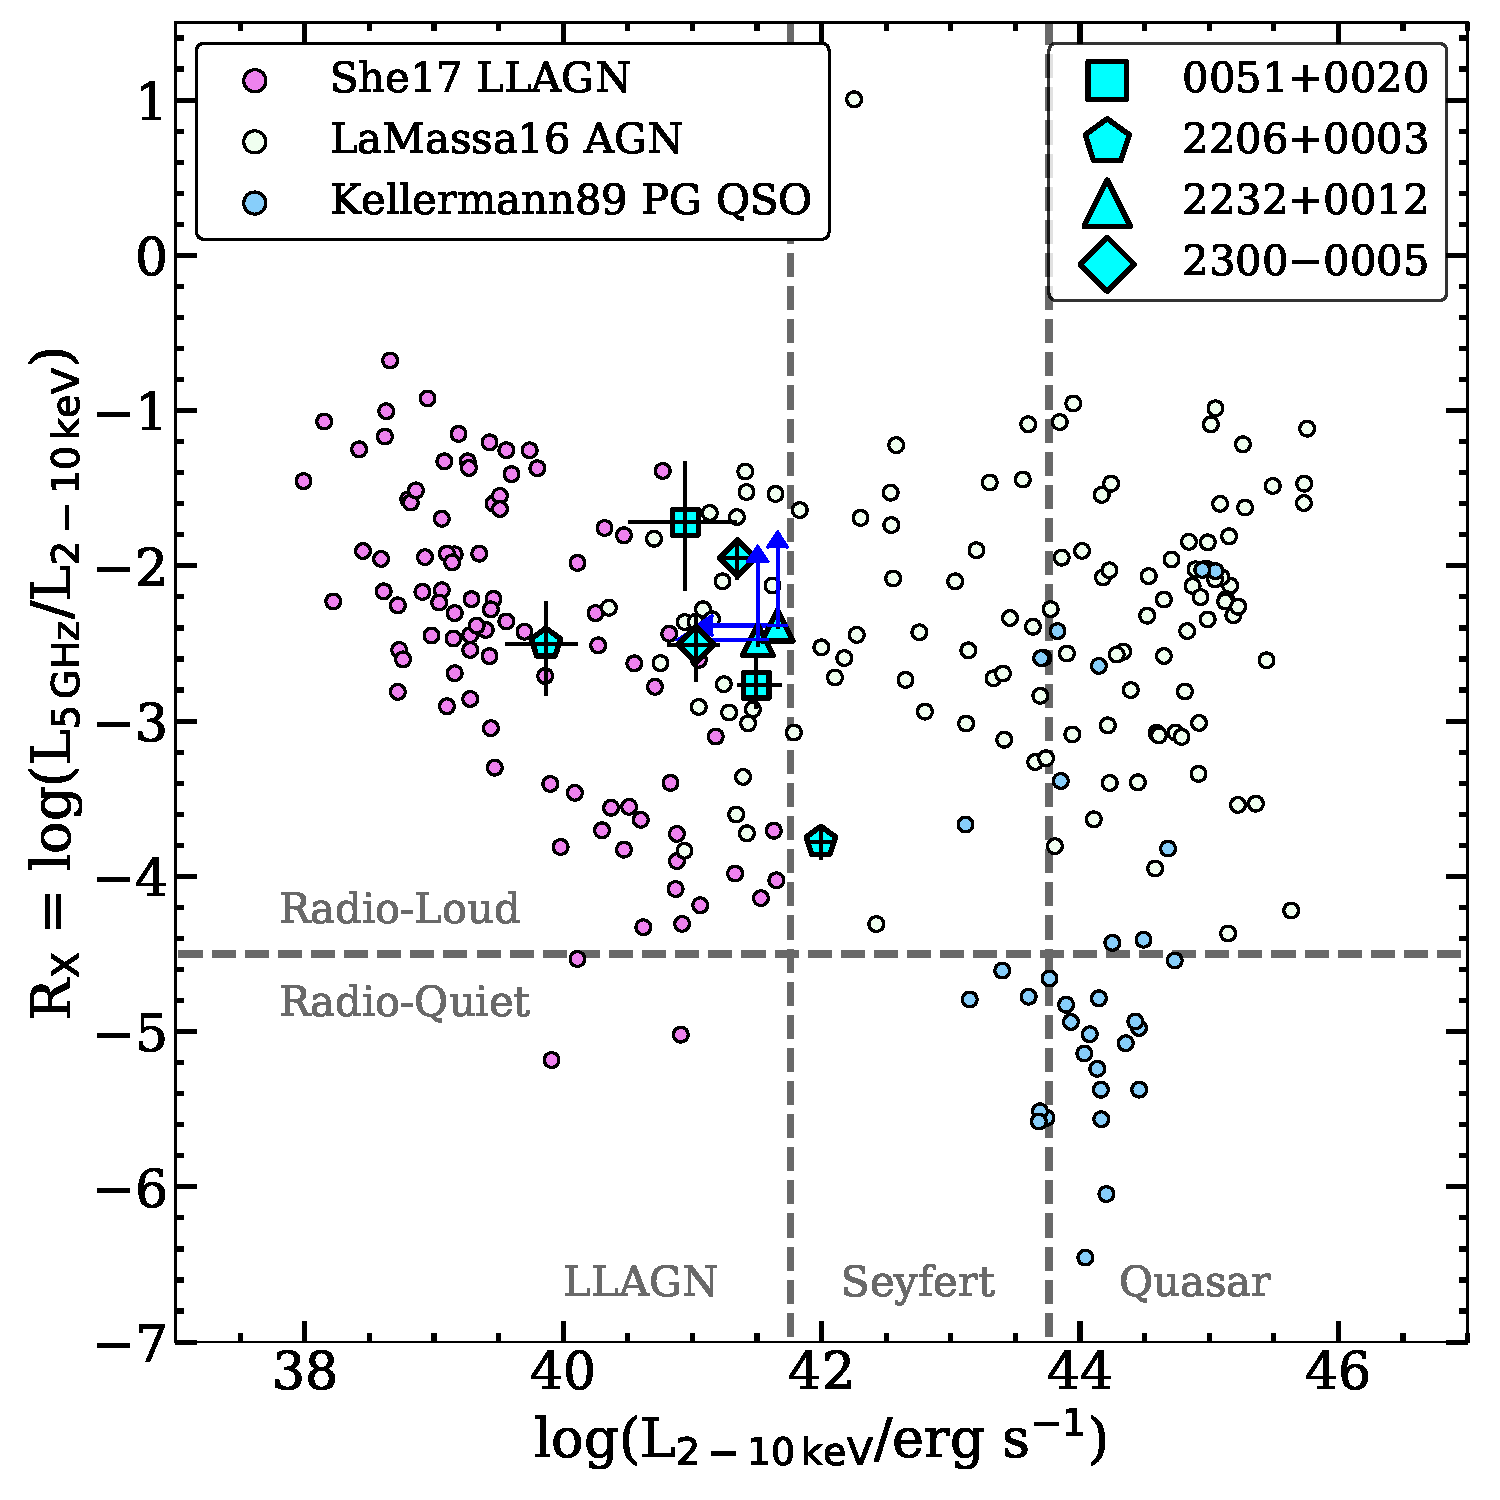
\includegraphics[width=8.5cm]{figs/Rx_Lx.pdf}
\caption{Radio-to-X-ray luminosity ratio ($R_{\rm X}$) vs. unabsorbed rest-frame 2-10\,keV luminosity (\lx). The large cyan symbols represent the components in the dAGNs, where the symbol shapes denote object designation as labelled in the legend at the upper right corner. The small color-filled circles show the comparison samples described in \S\,\ref{sec:Lx} and labeled in the legend on the upper left. The vertical dashed lines at $\log (L_{\rm X}/{\rm erg\,s}^{-1}) = 41.76$ and $43.76$ roughly divide AGNs into three luminosity regimes: LLAGN, Seyfert, and Quasar \citep{Brusa07}. The horizontal dashed line separates radio-loud ($R_{\rm X} > -4.5$) and radio-quiet ($R_{\rm X} < -4.5$) AGNs. The dAGNs have X-ray luminosities in the LLAGNs regime and show similar radio-to-X-ray ratios.}
\label{fig:Rx}
\end{figure}

The AGNs in our sample have X-ray luminosities in the range of $39.8 <$ log$\,L_{\rm X}/{\rm erg~s}^{-1} < 42.0$, which is in the regime between nearby LLAGNs and Seyferts \citep{Ho08}. In this section, we compare the dAGNs with other low-redshift AGNs in terms of general AGN properties, such as radio-to-X-ray ratio, BH fundamental plane, and Eddington ratio. We find that the dAGNs are similar to nearby LLAGNs, indicating that being involved in close galactic encounters does not affect these general AGN properties. 

In Fig.~\ref{fig:Rx}, we plot $R_{\rm X}$, the radio-to-X-ray luminosity ratio defined as $R_{\rm X} \equiv \log(L_{\rm 5GHz}/L_{\rm X})$, against $L_{\rm X}$, the unabsorbed X-ray luminosity in rest-frame 2-10\,keV. Here the monochromatic radio luminosity is defined as $\nu L_\nu$ at rest-frame 5\,GHz.
%
To compare our dAGNs with the general AGN populations, we show three comparison samples from the literature in Fig.\,\ref{fig:Rx}.
%  
First, we adopt the X-ray luminosities of a sample of nearby ($< 50$ Mpc) LLAGNs from \citet{She17} to populate the low luminosity regime ($L_{\rm X} \lesssim 10^{42}$\,\ergs). To calculate the radio luminosities of the LLAGNs, we cross-matched the X-ray catalog with the FIRST 1.4\,GHz catalog \citep{Helfand15} with a matching radius of $7\arcsec$ \citep{Lamassa16}, and then extrapolated the 1.4\,GHz flux density to 5\,GHz assuming a spectral index of $\alpha = 0.7$. 
%
Second, we adopt the X-ray luminosities and 1.4\,GHz radio fluxes of the X-ray-selected AGNs from the multi-wavelength catalog of the Stripe 82 X-ray Survey \citep{Lamassa16} to populate the Seyfert regime ($10^{42} \lesssim L_{\rm X} \lesssim 10^{44}$\,\ergs). Similar to the LLAGN sample, a $K$-correction was applied to the 1.4\,GHz flux density assuming $\alpha = 0.7$. We also $K$-correct the observed luminosities in 0.5-7\,keV (\chandra) and 0.5-10\,keV (\xmm) to rest-frame 2$-$10 keV assuming $\Gamma = 1.9$.
%
Lastly, we include a subset of Palomar-Green QSOs, for which we compiled 5\,GHz fluxes from \citet{Kellermann89} and \xmm\ X-ray luminosities from \citet{Piconcelli05}. 

Fig.\,\ref{fig:Rx} suggests that the dAGNs show similar radio-to-X-ray ratios as the LLAGNs and Seyferts, but are distinct from the PG QSOs which are mostly radio quiet. This shows that the dAGNs follow the same radio-X-ray scaling relation established by the general AGN population that are mostly hosted by isolated galaxies. On the other hand, $R_{\rm X}$ is directly related to the radio-to-X-ray spectral index between 5\,GHz and 2\,keV ($4.84\times10^{17}$\,Hz):
\begin{equation}
 \alpha_{\rm RX} = (R_{\rm X}+8.242)/8 ~~~{\rm for}~~~ \Gamma = 1.9.
\end{equation}
For the average value of $R_{\rm X} = -2.5$, $\alpha_{\rm RX}$ equals 0.72, consistent with a single synchrotron spectrum extending from X-ray to radio \citep[e.g.,][]{Hardcastle01}. Nonetheless, this crude SED slope measurement is inadequate to rule out models that predict separate origins of the X-ray and the radio emission. 

\begin{figure}
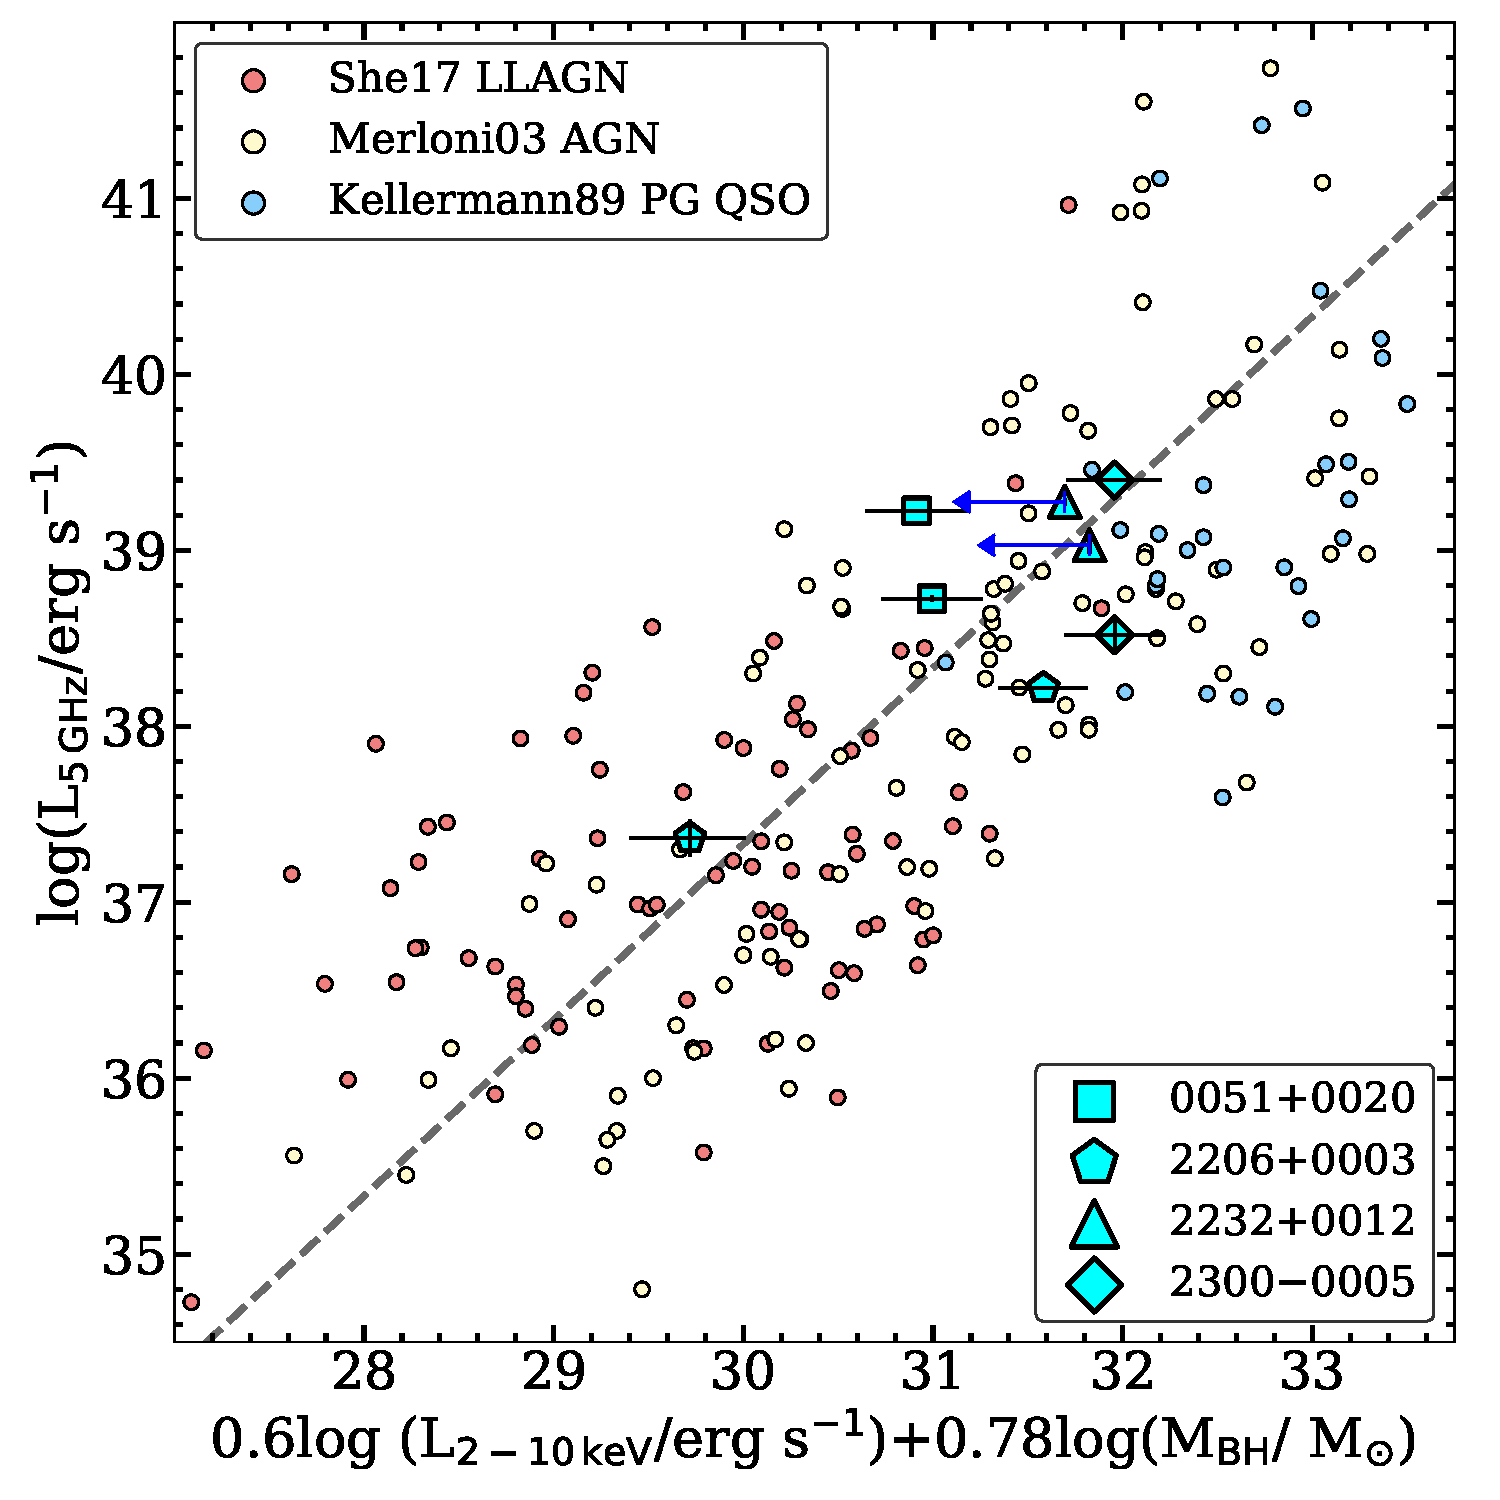
\includegraphics[width=8.5cm, height=8.5cm]{figs/BHFP.pdf}
\caption{The black hole fundamental plane \citep{Merloni03}. The dashed line follows the empirical relation given in Eq.~\ref{eq:BHFP}. The cyan points for our sample follow the same convention as in Fig.~\ref{fig:Rx}. The arrows indicate X-ray upper-limits. The smaller data points show the comparison samples described in \S\,\ref{sec:Lx}. Our dAGN follow well the fundamental plane relation with no systematic offsets.}
\label{fig:BHFP}
\end{figure}

Furthermore, the radio$-$X-ray correlation is closely related to the BH fundamental plane, which is established by both stellar-mass BHs in the Galaxy and the SMBHs in AGNs and QSOs. The three-parameter empirical correlation is best-fit by the following power-law \citep{Merloni03}:
\begin{multline}
\log(L_{\rm 5GHz}/{\rm erg\,s}^{-1}) =  \\
0.6 \log(L_{\rm X}/{\rm erg\,s}^{-1}) + 0.78 \log(M_{\rm BH}/\rm M_\odot) + 7.33,
\label{eq:BHFP}
\end{multline}
where $L_{\rm 5GHz}$, $L_{\rm X}$, and $M_{\rm BH}$ are the rest-frame 5\,GHz luminosity of the radio core, rest-frame 2$-$10\,keV luminosity, and BH mass, respectively. Although the relation holds over an impressive range of BH mass and luminosity, it has a rather large scatter ($\sim$1\,dex) and both the disk-jet model \citep{Merloni03} and the jet-dominated model \citep{Falcke04} can explain the same correlation. 

With the X-ray luminosities from \chandra\ and the BH masses from the $M_{\rm BH}-\sigma_\star$ relation, we can now place the dAGNs on the fundamental plane in Fig.\,\ref{fig:BHFP}. Similar to Fig.\,\ref{fig:Rx}, we also plot the following comparison samples: (1) the AGNs from the original \citet{Merloni03} sample, (2) LLAGNs with \chandra/ACIS X-ray luminosity and BH mass from the $\rm M_{\rm BH}-\sigma_\star$ relation \citep{She17} and 1.4\,GHz radio flux from the FIRST survey \citep{Helfand15}, and (3) PG QSOs with 5\,GHz radio flux from \citet{Kellermann89}, \xmm\ X-ray luminosity from \citet{Piconcelli05}, and H$\beta$-based virial BH mass from \citet{Lani17}. It is clear from Fig.~\ref{fig:BHFP} that the dAGNs follow the same fundamental plane relation as the other AGN samples. They are distributed well within the scatter of the relation, with no systematic deviation from the best-fit relation. 

Lastly, multiplying \lx\ by $\sim$16 to estimate the bolometric luminosity \citep{Ho08} and using the $\sigma_\star$-derived BH mass to estimate the Eddington luminosity for pure ionized hydrogen, we find that the dAGNs have Eddington ratios between $-5 < \log L_{\rm bol}/L_{\rm Edd} < -3$, which again are similar to LLAGNs.

\subsection{Distribution of X-ray Hardness Ratios} \label{sec:HR}

Merger simulations suggest high gas column density in merging galaxies due to the central concentration of gas as the tidal interactions funnel the ISM into the central kpc \citep{Hernquist89}. Simulations done by \citet{Hopkins06b} predict a wide distribution of column densities ($N_{\rm H} = 10^{21} - 10^{25}$\,cm$^{-2}$) for a complete hard X-ray sample of quasars. The distribution peaks around $10^{23}$\,cm$^{-2}$, and contains a non-negligible population of Compton-thick ($10^{24}$\,cm$^{-2}$) quasars. Our \chandra\ observations offer a way to test these predictions. 
As described in \S~\ref{sec:photo}, we have obtained HR measurements for six sources in our dAGN sample. By assuming an unabsorbed photon index of the intrinsic AGN emission, the observed HRs can be used as a proxy for the column density, and we find that only one of the six sources are obscured (i.e., $N_{\rm H} > 10^{22}$\,cm$^{-2}$; see Table\,\ref{tab:xraydata}). In this subsection, we examine whether the distribution of the HR values is different from that of the general population of AGNs. 

To construct the control sample, we select 68 AGNs with X-ray luminosities between $39.8 < \log L_{\rm X}/{\rm erg\,s^{-1}} < 42.0$ from the catalog of 314 nearby LLAGN observed by \chandra\ \citep{She17}. The luminosity range matches that of the dAGNs, so it prevents potential biases of the HRs due to any possible correlation between $N_{\rm H}$ and $L_{\rm X}$. The control data set is an archival compilation obtained over many \chandra\ cycles, wherein the sensitivity of the detectors in soft X-ray is known to degrade over time. In addition, different detector arrays (ACIS-I vs. ACIS-S) were used in the archival observations. For a fair comparison with the HR values of the dAGNs, we institute correction factors to convert the reported HR values of the control sample to reflect the characteristics of ACIS-S in Cycle\,18 based on PIMMS v4.8e (\url{http://cxc.harvard.edu/toolkit/pimms.jsp}). 

\begin{figure}
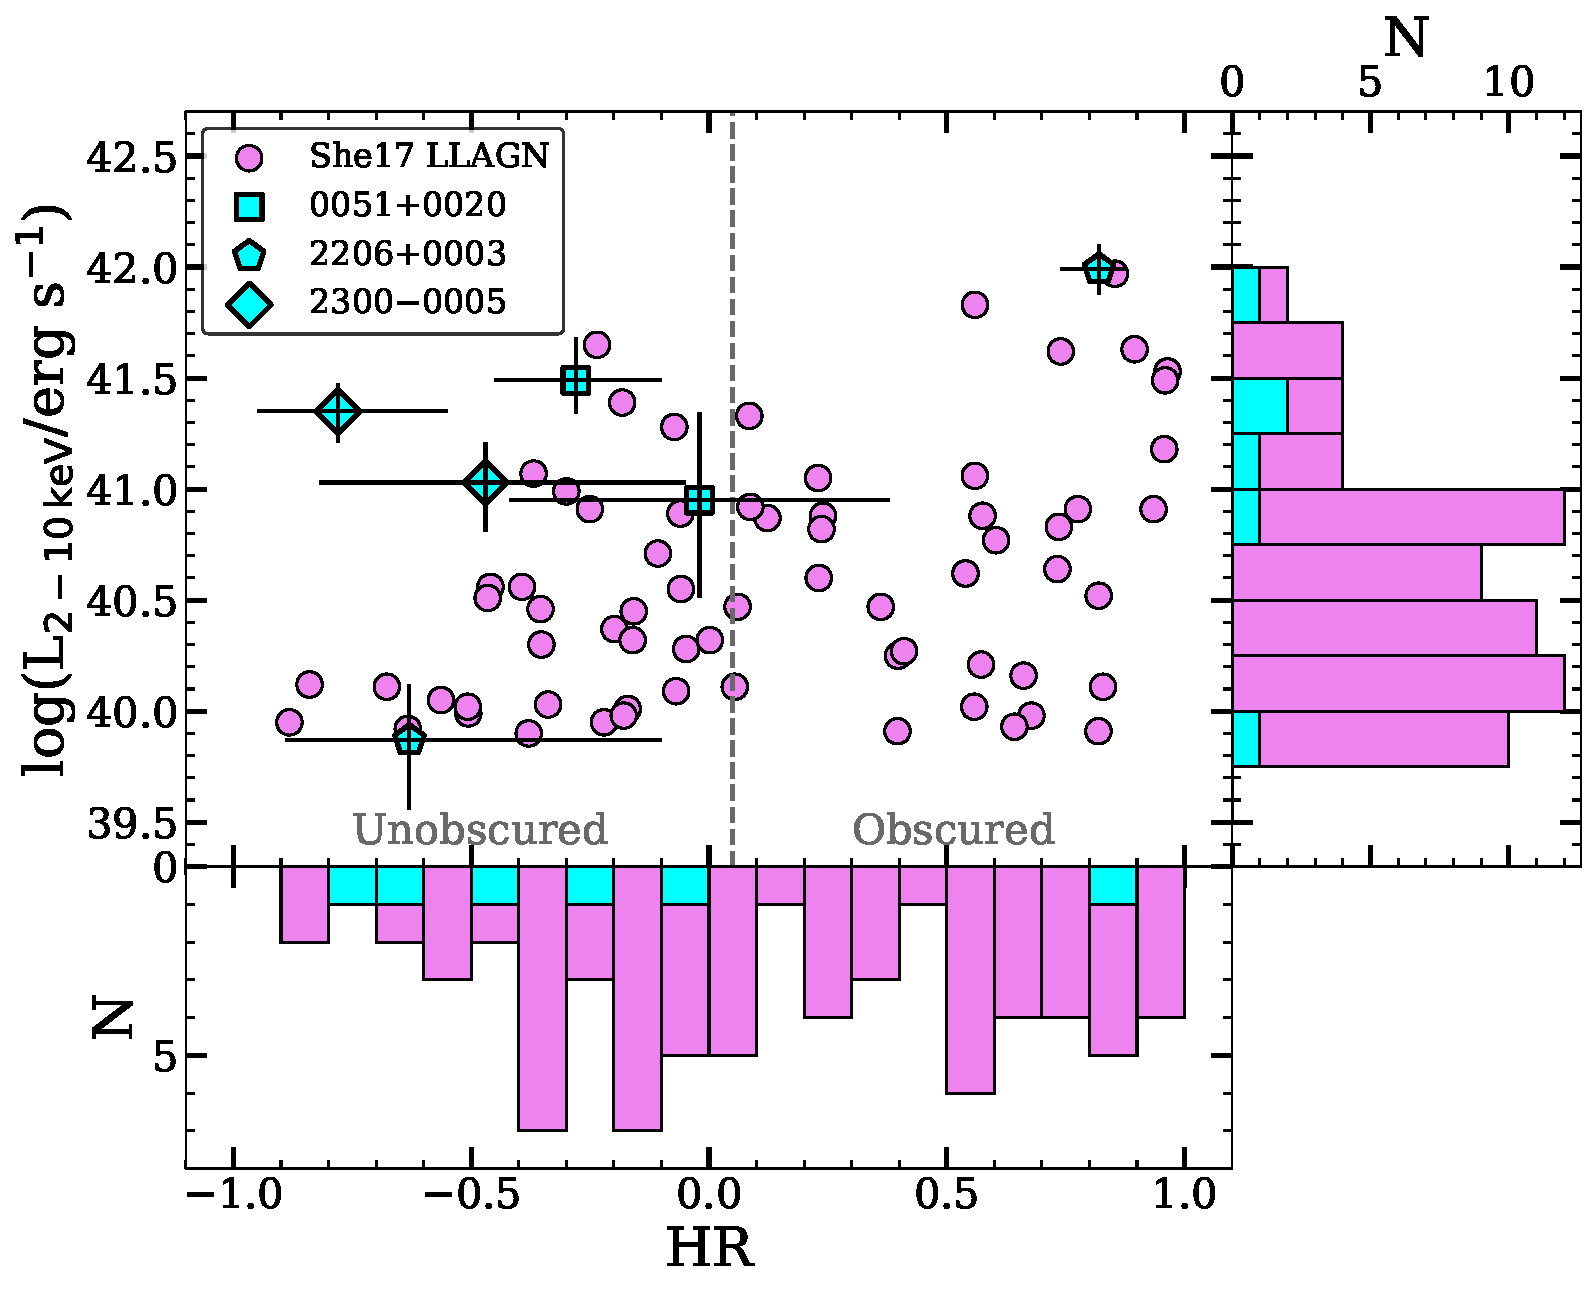
\includegraphics[width=8.5cm]{figs/triple_plot_scale.pdf}
\caption{X-ray luminosity vs. hardness ratio for our dAGNs ({\it cyan} points and histograms) and a control sample of nearby LLAGNs from \citet{She17} ({\it pink} points and histograms). A K-S test shows that the HR distribution of the dAGNs is consistent with that of the control sample. The vertical dashed line separates unobscured and obscured AGNs.}
\label{fig:HR_compare}
\end{figure}

In Fig.~\ref{fig:HR_compare}, we compare the distributions of the six X-ray detections in the dAGN sample and the control sample of LLAGNs in the plane of X-ray luminosity vs. HR. At first glance, the dAGNs appear to be systematically softer X-ray sources than the control sample, contrary to the expectation that merger-driven inflows produce higher X-ray obscurations in the host galaxies. Both X-ray sources in 2300$-$0005 are conspicuously soft compared to the control sample; as noted in \S~\ref{sec:photo}, their diffuse soft X-ray emission may originate from a circum-nuclear thermal plasma instead of nuclear accretion. Between $39.8 < \log L_{\rm X}/{\rm erg\,s^{-1}} < 42.0$, 36 out of the 68 LLAGNs in \citet{She17} have HR\,$> 0.05$, which corresponds to $N_{\rm H} > 10^{22}$\,\cmsq\ for $\Gamma = 1.9$. This fraction of obscured AGNs is consistent with the previously determined distribution of column densities as a function of X-ray luminosity from \citet{Ueda03}. In contrast, only one out of the six dAGN components have HR\,$> 0.05$. Limited by the small sample, the difference between the two obscured AGN fractions is $\sim$1.5$\sigma$ --- $53\pm6$\% vs. $17^{+23}_{-6}$\% --- where the 1$\sigma$ confidence intervals are estimated using the Bayesian approach for binomial population proportions \citep{Cameron11}. 

As a more quantitative comparison, we conduct a Kolmorogov-Smirnov (K-S) test between the HR distributions of the two samples. Based on the maximum deviation between two normalized cumulative distribution functions (the K-S statistic) and the sample sizes, the K-S test calculates the probability (i.e., the $p$-value) that two observed samples are drawn from the same parent sample. For the HR distributions of the two AGN samples, the $p$-value is 19\% because the K-S statistic is 0.43 and the sample sizes are 6 and 68. The $p$-value is much greater than the threshold value of $p$-value\,$<$\,5\%, indicating that the HR distributions of the dAGNs and the control sample are not sufficiently different. Therefore, the X-ray HRs of the dAGNs are normal for their luminosity, lending no evidence that X-ray emission is more obscured in galaxy mergers than in isolated AGNs, even when the projected separations are less than 12\,kpc.

\subsection{Elevated Obscuration or Contamination from Star Formation?} \label{sec:deficit}

Previous works report evidence that dAGNs show higher degrees of obscuration by comparing the X-ray luminosity with the [O\,{\sc iii}]\,$\lambda$5007 line luminosity \citep{Liu13a} or the mid-IR (12\,\um) luminosity \citep{Satyapal17}. In both cases, the observed X-ray luminosities of dAGNs are lower than expected from the other AGN luminosity tracers. In this subsection, we use the same diagnostic tools on the radio-selected dAGNs. 

\begin{figure*}
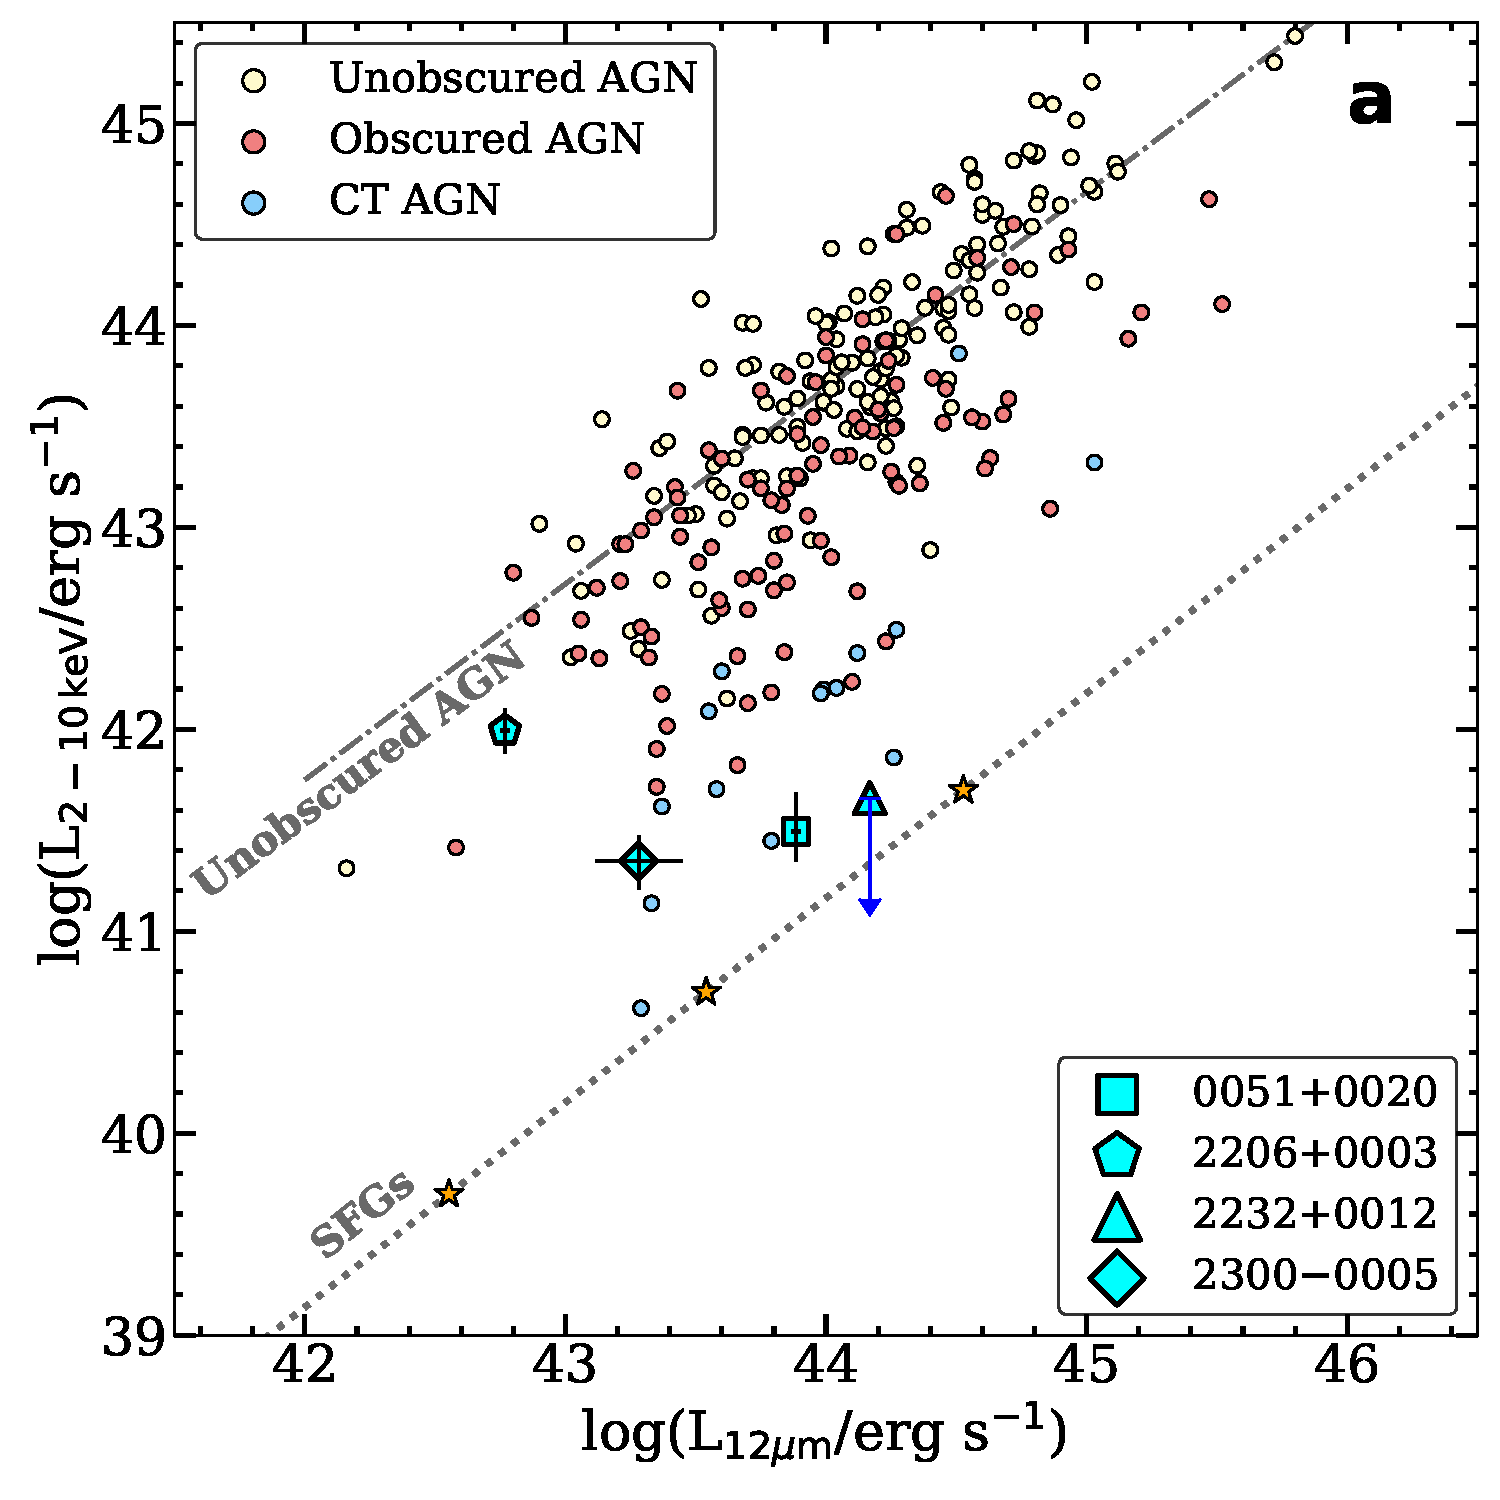
\includegraphics[width=8.5cm]{figs/Lx-Lir_rest.pdf}
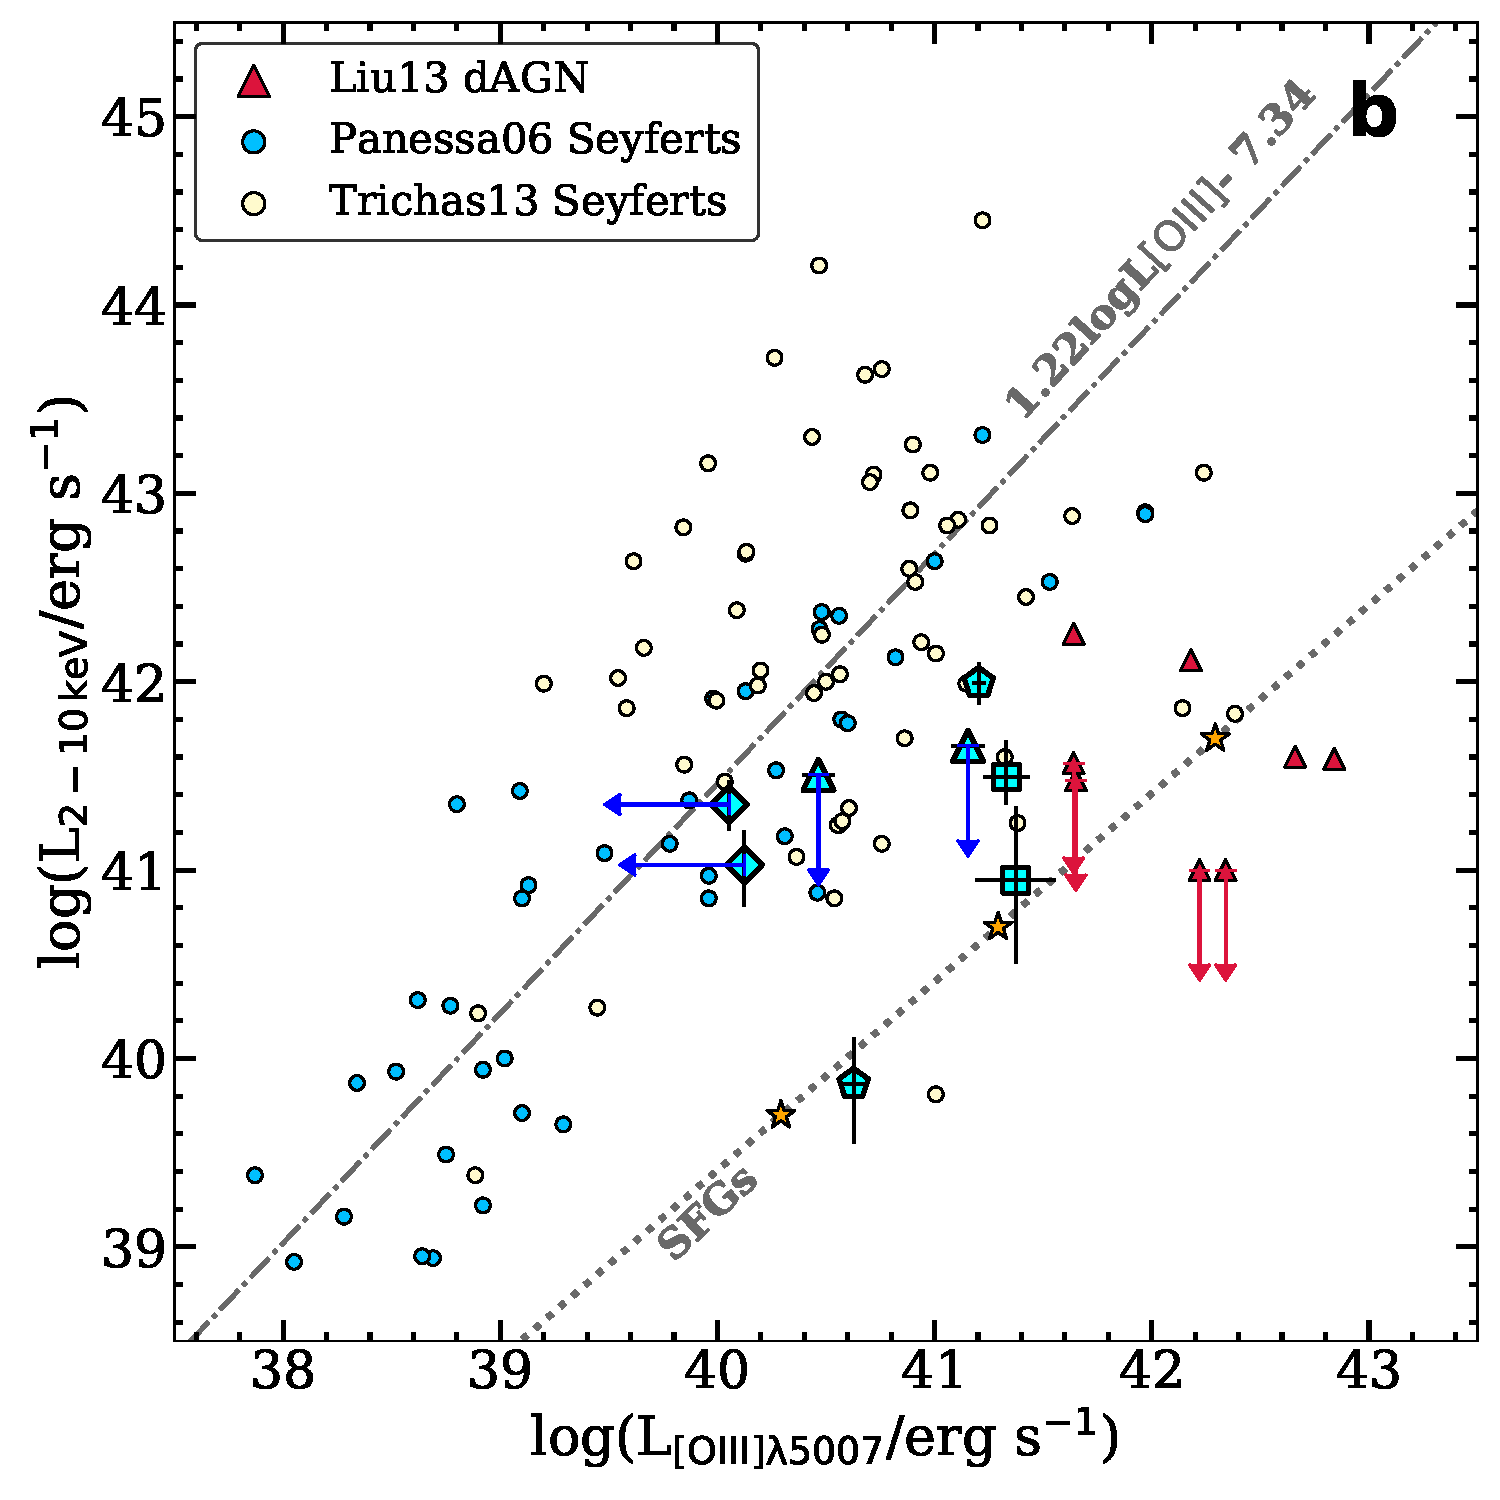
\includegraphics[width=8.5cm]{figs/Lx-L[OIII]unabs.pdf}
\caption{Luminosity relations sensitive to X-ray obscuration. 
%
({\it a}): $L_{\rm X}$ vs. rest-frame 12\,\um\ luminosity from WISE. The large cyan data points with error bars show our dAGNs and the small circles are BAT AGNs from \citet{Ricci15}. Due to the spatial resolution of WISE, the luminosities plotted for the dAGNs are the sum of both components in each dual system. The dotted line shows the expected relation for star-forming galaxies, with stars marking SFRs at 1 , 10, and 100\,\msunyr. 
%
({\it b}): $L_{\rm X}$ vs. extinction-corrected [O\,{\sc iii}]$\lambda$5007 line luminosity. Red triangles denote the dAGNs from \citet{Liu13} and the small circles show comparison samples of type-2 Seyferts compiled from \citet{Panessa06} and \citet{Trichas13}. 
%
The dAGNs show apparent X-ray deficits relative to the mid-IR and [O\,{\sc iii}] luminosities, which may be due to enhanced \lmir\ and \loiii\ from star formation instead of elevated X-ray obscuration.
}
\label{fig:LxLir}
\end{figure*}

In Fig.~\ref{fig:LxLir}$a$ we plot X-ray luminosity against mid-infrared luminosity, following \citet{Satyapal17}. For the dAGNs, we interpolate the AllWISE photometry\footnote{\url{http://wise2.ipac.caltech.edu/docs/release/allwise/expsup/}} from the Wide-field Infrared Survey Explorer (WISE) mission \citep{Wright10} to obtain the rest-frame 12\,\um\ luminosities ($L_{12\mu m}$). Because our dAGNs are spatially unresolved in WISE (FWHM $\sim$ 6\arcsec \  to 12\arcsec), the 12\,\um\ luminosity is that of the whole dAGN system rather than that of individual components. To be consistent, we plot the combined X-ray luminosity for each dAGN. For comparison with the general AGN population, we show the hard X-ray selected nearby AGNs from the 70 month Swift/BAT survey \citep{Baumgartner13, Ricci15}. The BAT AGNs are denoted as unobscured ($N_{\rm H} < 10^{22}$\,\cmsq), obscured ($10^{\rm 22} < N_{\rm H} < 10^{\rm 24}$\,\cmsq), or Compton-thick ($N_{\rm H} > 10^{\rm 24}$\,\cmsq), based on column densities estimated from X-ray spectral analysis. As previously observed, unobscured BAT AGNs follow a linear correlation between \lx\ and \lmir, while obscured and Compton-thick AGNs systematically deviate from this correlation by showing an apparent deficit in X-ray luminosity. This is because the mid-IR photons emitted by the circumnuclear torus are less affected by obscuration than the X-ray photons. This plot thus provides a diagnostic tool to identify obscured AGNs, albeit crude given the large scatter around the best-fit correlation. Similar to previously X-ray observed dAGNs compiled by \citet{Satyapal17}, the majority (3 out of 4) of the dAGNs in our sample fall systematically below the \lx-\lmir\ correlation established by unobscured AGNs. Ironically, the only obscured dAGN we identified based on the HR and the X-ray spectrum, 2206$+$0003, is in fact closest to the \lx-\lmir\ correlation. To elucidate this matter, we show the expected location of star-forming galaxies as a dotted line in Fig.~\ref{fig:LxLir}$a$, where we have used the \lmir-SFR relation from \citet{Donoso12} and the \lx-SFR relation from \citet{Ranalli03}:
\begin{align}
\log(L^{\rm SF}_{12 \mu m}/{\rm erg\ s^{-1}}) &= 0.987~\log({\rm SFR/M_\odot\ yr^{-1}}) + 42.5 \\
\log(L^{\rm SF}_{\rm 2-10 keV}/{\rm erg\ s^{-1}}) &= \log({\rm SFR/M_\odot\ yr^{-1}}) + 39.7
\label{eq:Lsf1}
\end{align}
Unsurprisingly, star-forming galaxies show a $\sim$2.3\,dex offset in \lx\ at any given \lmir. So an alternative way to explain the location of the dAGNs is that their mid-IR emission is dominated by star formation. This boosted mid-IR luminosity, if interpreted as intrinsic to the AGN, would misdiagnose a supposed lack of X-ray luminosity as being due to absorption by enhanced obscuration. Therefore, while our dAGNs do fall below the trend for unobscured AGN, the mid-IR contribution from star formation (in 0051$+$0020, 2206$+$0003, and 2232$+$0012) and the X-ray contribution from non-nuclear hot ISM (in 2300$-$0005) offer alternative interpretations other than enhanced X-ray obscuration for the observed offsets.

By comparing \lx\ with the H$\alpha$ luminosity, we find that for two objects in our sample, 0051$+$0020NE and 2206$+$0003NW, the H$\alpha$-inferred SFR ($\sim$1-10 \msunyr) may explain the bulk of the X-ray luminosity $\rm L_{\rm X}$, consistent with their BPT classifications as AGN-star-forming composite galaxies \citepalias{Fu15a}. The remaining four X-ray-detected objects all require an additional source of X-ray emission beyond star formation, most likely nuclear accretion. Interestingly, star-forming galaxies have similar radio-to-X-ray ratios as the LLAGNs in Fig.\,\ref{fig:Rx}. We obtain $R_{\rm X} = -2.2$ using the $L_{\rm 1.4\ GHz}$-SFR relation from \citet{Murphy11} and the \lx-SFR relation from \citet{Ranalli03}:
\begin{align} 
\Big(\frac{\rm SFR}{{\rm M_{\odot}\ yr^{-1}}}\Big) &= 6.35 \times 10^{-29} \Big(\frac{L_{\rm 1.4\ GHz}^{\rm SF}}{\rm erg\ s^{-1}\ Hz^{-1}}\Big) \\
\Big(\frac{\rm SFR}{{\rm M_{\odot} \ yr^{-1}}}\Big) &= 2.0\times10^{-40} \Big(\frac{L_{\rm 2-10keV}^{\rm SF}}{\rm erg\ s^{-1}}\Big)    
\label{eq:SFR}
\end{align} 

The [O\,{\sc iii}]\,$\lambda$5007 line emission from the AGN narrow-line region is less affected by obscuration than the nuclear X-ray emission region because it is spatially extended on kpc-scales. This makes the X-ray to [O\,{\sc iii}] luminosity ratio another diagnostic tool to identify obscured AGNs \citep{Panessa06}. \citet{Liu13} found that the X-ray to [O\,{\sc iii}] luminosity ratios of double-peaked [O\,{\sc iii}]-selected dAGNs are systematically lower than those of optically selected single type-2 AGNs, by as much as $\sim$2\,dex. They suggest that the dAGNs are systematically X-ray weak because of higher X-ray absorption columns and/or a viewing angle bias from the double-peak selection. We reproduce the \lx\ vs. \loiii\ plot in Fig.\,\ref{fig:LxLir}$b$ to check whether our dAGN are similarly X-ray weak compared to their [O\,{\sc iii}] luminosity. We measure the [O\,{\sc iii}] luminosity of our dAGNs using the optical spectra from either SDSS or Keck, corrected for both the dust extinction using the Balmer decrement as well as the aperture loss \citepalias{Fu15b}. 
%
To compare the dAGNs from our sample and that of \citet{Liu13} with the general AGN population, we also show comparison samples of low-redshift Seyfert-2s from \citet{Panessa06} and \citet{Trichas13}. The [O\,{\sc iii}] luminosities of the two samples are from the Palomar Survey of nearby galaxies \citep{Ho97a} and the MPA-JHU spectral measurements for the SDSS spectra\footnote{\url{https://wwwmpa.mpa-garching.mpg.de/SDSS/DR7/}}, respectively. 
%
Both dAGN samples lie systematically below the mean relation established by the comparison samples, although the radio-selected dAGNs are less offset than the double-peak-selected dAGNs because of their lower [O\,{\sc iii}] luminosities. In fact, given the large scatter of the \lx-\loiii\ relation, most of our dAGNs are within $\sim$2$\sigma$ of the mean relation.   

Similar to the \lx-\lmir\ diagnostic, the apparent X-ray deficiency relative to the [O\,{\sc iii}] luminosity can also be explained by the emission-line contribution from other ionization sources, such as star formation, radiative shocks, and evolved stellar populations. We show in Fig.\,\ref{fig:LxLir}$b$ the \lx-\loiii\ relation of pure star-forming galaxies as a dotted line, where we have used the \lx-SFR relation in Eq.\,\ref{eq:Lsf1} and the $L_{\rm H\alpha}$-SFR relation from \citet{Murphy11}: 
\begin{equation}
\log(L^{\rm SF}_{\rm H\alpha}/{\rm erg\ s^{-1}}) = \log({\rm SFR/M_\odot\ yr^{-1}}) + 41.3
\label{eq:lsf2}
\end{equation}
The H$\alpha$ luminosity is then converted to \loiii\ assuming emission-line ratios of H$\alpha$/H$\beta$ = 2.85 and [O\,{\sc iii}]/H$\beta$ = 0.3, typical for star-forming galaxies with $M_\star \sim 10^{10}$\,\msun. The \lx-\loiii\ relation of star-forming galaxies falls $\sim$2.5\,dex below that of Seyfert-2s. The apparent X-ray deficiency can thus be explained by the star-forming contribution to \loiii.

\section{Summary and Conclusion} \label{sec:summary}

Previously we have identified four dAGNs at $z \sim 0.1$ and projected separations between 4\,kpc and 12\,kpc in the SDSS Stripe 82 field with VLA imaging and optical spectroscopy. In this work, we have obtained \chandra\ ACIS-S observations of the dAGNs and detected X-ray emission from six of the eight dAGN components at $>$3$\sigma$ confidence level. The X-ray and multi-wavelength properties of the dAGNs are analyzed and compared with the general AGN population and previously studied dAGNs compiled from the literature. Our main results are summarized below:

\begin{enumerate}

\item The intrinsic rest-frame 2$-$10\,keV luminosities of our sample ranges between $39.8 < \log\,L_{\rm X}/{\rm erg~s}^{-1} < 42.0$, straddling the luminosity boundary between nearby LLAGNs and Seyferts. With $7.4 < \log M_{\rm BH}/M_\odot < 9.4$ and $37.4 < \log L_{\rm 5 GHz}/{\rm erg~s}^{-1} < 39.4$, the components in the dAGNs show low Eddington ratios and high radio-to-X-ray luminosity ratios similar to those of LLAGNs, and they follow the same BH fundamental plane relation as the general AGN population. 

\item The X-ray hardness ratios indicate one obscured AGN among the six X-ray detected sources with $\log N_{\rm H}/{\rm cm}^{-2} = 22.7$. X-ray spectral fitting of this source finds a similarly high column density of $\log N_{\rm H}/{\rm cm}^{-2} = 23.1$. Based on HR-inferred column densities, the fraction of obscured AGNs ($17^{+23}_{-6}$\%) in the dAGN sample is in fact {\it lower} than that of nearby LLAGNs in the same luminosity range ($53\pm6$\%). Despite the large statistical uncertainties, this result is at odds with simulation predictions of enhanced obscuration in advanced mergers due to large-scale gas inflows.

\item The dAGNs show apparent X-ray deficiency with respect to the AGN luminosities inferred from the 12\,\um\ WISE photometry and the [O\,{\sc iii}] spectroscopy, similar to previously studied dAGNs selected using other techniques. But it is important to account for the contribution from star formation when interpreting the ``X-ray deficit,'' because the AGN luminosities inferred from mid-IR continuum and optical emission lines may have been significantly overestimated without subtracting the star-forming component. 

\end{enumerate}

Considering the multi-wavelength evidence, the radio-selected dAGNs in Stripe 82 show properties similar to nearby LLAGNs in terms of radio-to-X-ray ratio, the Eddington ratio, and BH mass. At odds with previous claims, we find that obscured AGNs are rare among dAGNs based on X-ray HR measurements. Although apparent X-ray deficiency is observed relative to mid-IR or [O\,{\sc iii}] luminosities in the dAGNs, significant contribution to \lmir\ and \loiii\ from star formation (i.e., mid-IR and emission-line excess) provides a more natural explanation for the data. This alternative interpretation is also more consistent with (1) the agreement with the BH fundamental plane (\S~\ref{sec:Lx}), (2) the normal X-ray HR distribution (\S~\ref{sec:HR}), and (3) the AGN$-$star-forming composite emission-line ratios in the BPT diagram \citepalias[see][Fig.~6]{Fu15a}.

Therefore, our observations of the radio-selected dAGNs show that being involved in close galactic encounters does not significantly alter the general AGN properties nor does it increase the X-ray obscuring column density. These results seem to be in tension with the merger-driven scenario of AGN fueling, especially given that (1) these galaxies are in kpc-scale mergers, (2) at least two of the dAGNs show spectacular tidal tails and shells that indicate a post-pericentric encounter, and (3) the number of observed dAGNs exceeds by an order-of-magnitude the expectation from random pairing and the mean duty cycle of radio AGNs in VLA-Stripe82 \citepalias[3 observed vs. 0.3 expected $(13\times(551/22192))$; see][\S\,3.4]{Fu15b}. 

To reconcile these results, the most promising feeding mechanism to explain the low-level AGN activities in our dAGNs is probably stochastic-mode accretion due to tidally-triggered minor perturbations \citep[e.g.,][]{Hopkins06a}. In contrast to the conventional ``merger-driven accretion'' where the SMBH accretion is fueled by kpc-scale gas inflows and regulated by feedback \citep[e.g.,][]{Di-Matteo05,Hopkins05a}, the stochastic accretion naturally explains the similarities between the dAGNs and LLAGNs in apparently non-interacting hosts and the high frequency of correlated AGNs (thus the higher-than-expected number of dAGNs), but it evades the problem of enhanced obscuring column density due to large-scale tidal inflows (which is unobserved in our sample). Because a LLAGN with $L_{\rm bol} \lesssim 10^{10}$\,\lsun\ with a lifetime of 10\,Myr only requires a modest amount of gas supply ($M \lesssim 6\times10^4/(\eta_{\rm rad}/0.1)$\,\msun, where $\eta_{\rm rad}$ is the radiative efficiency), large-scale gravitational torques from major mergers are not required to deliver the gas into the galactic nuclei. Instead, a sufficient amount of gas can be delivered to the nuclei even by a low-level cooling flow of the hot ISM in hydrostatic equilibrium \citep[e.g.,][]{Allen06}, and minor perturbations such as disk and bar instabilities \citep[e.g.,][]{Norman83,Jogee06}, magnetic breaking \citep[e.g.,][]{Krolik90}, $N$-body cloud-cloud or cloud-cluster interactions like in the Galactic center \citep[e.g.,][]{Genzel94}, and minor mergers \citep[e.g.,][]{Hernquist95}. Once the nuclear gas reservoir has been built up, the BH can accrete gas through stochastic cloud collisions, and the accretion is subsequently self-regulated by feedback \citep[e.g.,][]{Yuan11,Bu19} . This stochastic accretion mode is distinct from the major-merger-induced accretion mode, and the former dominates the latter in the AGN population below the Seyfert/Quasar transition luminosity of $L_{\rm bol} = 10^{12}$\,\lsun\ \citep{Hopkins14a}. The low-level AGNs in major mergers in our sample show that the stochastic mode continues to operate even in the presence of large-scale tidal torques. The gas-rich major mergers may not have induced kpc-scale gas inflows (which would have obscured the X-ray), but they may have triggered minor perturbations in both nuclei simultaneously, which led to the high fraction of correlated LLAGNs in mergers. Therefore, we believe most of the dAGNs identified to date can be explained as merger-synchronized stochastic accretion; the SMBHs in these dAGNs are probably not fueled by large-scale gas inflows induced by tidal torques.

\acknowledgments

We thank our colleagues Philip Kaaret, Joshua Steffen, and Dylan Par\'e for helpful discussions. We also thank Shobita Satyapal, Claudio Ricci, and Magdalena Kunert-Brajraszewska for providing data from their previous analyses. 
% DATA
The scientific results reported in this article are based on observations made by the Chandra X-ray Observatory.
% Funding
Support for this work was provided by the National Aeronautics and Space Administration (NASA) through Chandra Award Number GO7-18084X issued by the Chandra X-ray Center, which is operated by the Smithsonian Astrophysical Observatory for and on behalf of the National Aeronautics Space Administration under contract NAS8-03060.
% additional funding
We also acknowledge support from the National Science Foundation (NSF) grant AST-1614326. 
%author-specific funding
S.G.D. also acknowledges partial support from NSF grants AST-1413600 and AST-1518308, as well as NASA grant 16-ADAP16-0232. A.D.M. acknowledges partial support from NSF grant 1616168. 
% software
This research has made use of software provided by the Chandra X-ray Center (CXC) in the application packages CIAO, ChIPS, and Sherpa.

%%%%%%%%%%%%%%%%%%%% REFERENCES %%%%%%%%%%%%%%%%%%
\bibliographystyle{aasjournal}
\bibliography{exgal_ref}

\end{document}